% !TeX program = xelatex
\documentclass[runningheads]{llncs}
\usepackage[paperheight=295mm,paperwidth=210mm]{geometry}
\usepackage{graphicx}
\usepackage{wrapfig}
\usepackage{import}
\usepackage{kotex}
\usepackage[dvipsnames]{xcolor}
\usepackage{fancyvrb} %
\usepackage{listings}
\usepackage{tabularx}
\usepackage{underscore}
\usepackage{multicol}
\usepackage{enumitem}
\usepackage{subcaption}
\usepackage[numbers,square,super]{natbib}
\usepackage{mathptmx} % Times New Roman
\usepackage{amsmath}
\usepackage{amssymb}
\usepackage{framed}
\usepackage{etoolbox}
\usepackage{cancel}
\usepackage{physics}
\usepackage{tikz}
\usepackage{parskip}
\usepackage{enumerate}
\usepackage{minted}
\usepackage{inconsolata}
\usepackage{makecell}
\usepackage{slashed}
\usepackage{nicematrix}
\usetikzlibrary{calc, angles, quotes, graphs, positioning, arrows}

\setcounter{tocdepth}{2}

\colorlet{shadecolor}{gray!30}

\newcommand\enclosebox[2]{%
  \BeforeBeginEnvironment{#1}{\begin{#2}}%
  \AfterEndEnvironment{#1}{\end{#2}}%
}

\enclosebox{theorem}{oframed}
\enclosebox{definition}{leftbar}

\newcommand{\divides}{\bigm|}
\newcommand{\ndivides}{%
  \mathrel{\mkern.5mu % small adjustment
    % superimpose \nmid to \big|
    \ooalign{\hidewidth$\big|$\hidewidth\cr$\nmid$\cr}%
  }%
}
\newcommand{\ord}{\operatorname{\mathrm{ord}}}
\newcommand{\ind}{\operatorname{\mathrm{ind}}}
\newcommand{\legendre}[2]{\left(\frac{#1}{#2}\right)}
\setmainfont{Times New Roman}
\setmainhangulfont{Nanum Myeongjo}
\setmonofont{SF Mono}
\setlength{\parindent}{1em}
\setlength{\parskip}{0pt}
\linespread{1.2}
%\renewcommand{\arraystretch}{1.5}
\setlength{\tabcolsep}{0.5em}%
\newenvironment{Figure}
  {\par\medskip\noindent\minipage{\linewidth}}
  {\endminipage\par\medskip}
\newcommand{\translation}[1]{\textsuperscript{#1}}

\makeatletter
\renewcommand\NAT@citesuper[3]{\ifNAT@swa
\if*#2*\else#2\NAT@spacechar\fi
\unskip\kern\p@\textsuperscript{\NAT@@open#1\if*#3*\else,\NAT@spacechar#3\fi\NAT@@close}%
   \else #1\fi\endgroup}
\makeatother

\let\oldtabular\tabular% Store a copy of \tabular
\let\endoldtabular\endtabular% Store a copy of \endtabular
\renewenvironment{tabular}[2][\arraystretch]
  {\edef\arraystretch{#1}% Update \arraystretch
   \oldtabular{#2}}% \begin{tabular}[<stretch>]{<col spec>}
  {\endoldtabular}% \end{tabular}

\begin{document}

\title{Discrete Mathematics (0034)\newline\space Final Exam Lecture Notes}
\author{Yulwon Rhee (202211342)}
\institute{Department of Computer Science and Engineering, Konkuk University}

\maketitle
\setcounter{section}{8}
\section{Week 9}
\subsection{관계}
\begin{itemize}
    \item 서로 다른 두 집합에 속하는 원소들 간의 순서\textsuperscript{Order}를 표현
    \item 순서쌍 집합(곱집합의 부분 집합)에 속하면서 순서쌍을 이루는 원소들은 `관계'가 있다
\end{itemize}

\subsection{이항 관계\textsuperscript{Binary Relation}}
집합 $A$에서 집합 $B$로 가는 관계\\
$R$: $A \times B$의 부분 집합\\
$a \in A, b \in B$일 때, $(a, b) \in R \to {_aR_b}$; $(a, b) \not\in R \to {_a\slashed{R}_b}$
\\\\
정의역\textsuperscript{Domain}: $\mathrm{dom}(R) = \{a | a \in A\}$\\
공변역\textsuperscript{Codomain}: $\mathrm{codom}(R) = \{b | b \in B\}$\\
치역\textsuperscript{Range}: $\mathrm{ran}(R) = \{b | (a, b) \in R\} \subseteq B$
\\\\
$n$항 관계\textsuperscript{$n$-ray Relation}: $R \subseteq A_1 \times A_2 \times \cdots \times A_n$의 부분 집합
\\\\
역관계\textsuperscript{Inverse Relations}: $B$에서 $A$로의 관계, $R^{-1} = \{(b, a) | (a, b) \in R\}$, $_aR_b$ 존재 $\to {_bR^{-1}_a}$ 존재

\subsection{관계의 표현: 서술식 방법}
e.g.) $A={1, 2, 3}$에서 원소 $a, b$가 $a \geq b$인 관계 $R$

\subsection{관계의 표현: 나열식 방법}
\begin{itemize}
    \item 화살표 도표\textsuperscript{Arrow diagram}
    \item 좌표 도표\textsuperscript{Coordinate diagram}:
          \begin{itemize}
              \item 집합 $A$의 원소를 $x$축 위의 점으로, $B$의 원소를 $y$축 위의 점으로 표시
          \end{itemize}
    \item 방향 그래프\textsuperscript{Directed graph}:
          \begin{itemize}
              \item 관계 $R$이 하나의 집합 $A$에 대한 관계 표현일 때
              \item $A$의 각 원소 $\Rightarrow$ 그래프의 정점\textsuperscript{Vertex}
              \item $(a, b) \in R$이면 $a$에서 $b$로 화살표가 있는 연결선\textsuperscript{Edge}로 표현
          \end{itemize}
    \item 관계 행렬\textsuperscript{Relation matrix}:
          \begin{itemize}
              \item 부울\textsuperscript{Boolean} 행렬 이용
              \item $A = \{a_1, a_2, \cdots, a_m\}$에서 $B = \{b_1, b_2, \cdots, b_n\}$로 가는 관계 $R$에 대한 $m \times n$ 행렬 $M_R=[m_{ij}]$
                    $$m_{ij} = \begin{cases}
                            1, (a_i, b_j) \in R \\
                            0, (a_i, b_j) \not\in R
                        \end{cases}$$
              \item e.g.) $A=\{1, 2, 3\}$과 $B=\{a, b\}$의 이항 관계

                    $R = \{(1, b), (2, a), (2, b), (3, a)\}$
                    $$M_R=\begin{bNiceMatrix}[first-row, first-col]
                              & a & b \\
                            1 & 0 & 1 \\
                            2 & 1 & 1 \\
                            3 & 1 & 0
                        \end{bNiceMatrix}\quad\quad\quad
                        M_{R^{-1}}=\begin{bNiceMatrix}[first-row, first-col]
                              & 1 & 2 & 3 \\
                            a & 0 & 1 & 1 \\
                            b & 1 & 1 & 0
                        \end{bNiceMatrix}$$
          \end{itemize}
\end{itemize}

\subsection{관계의 성질}
반사 관계\textsuperscript{Reflexive Relation}: 모든 $a \in A$에 대해 $(a, a) \in R$인 관계,
$\begin{bmatrix}
        1 &   &        &   \\
          & 1 &        &   \\
          &   & \ddots &   \\
          &   &        & 1
    \end{bmatrix}$\\
비반사 관계\textsuperscript{Irreflexive Relation}: 모든 $a \in A$에 대해 $(a, a) \not\in R$인 관계,
$\begin{bmatrix}
        0 &   &        &   \\
          & 0 &        &   \\
          &   & \ddots &   \\
          &   &        & 0
    \end{bmatrix}$\\
반사 관계도 비반사 관계도 아닌 경우: $\begin{bmatrix}
        0 &   &        &   \\
          & 1 &        &   \\
          &   & \ddots &   \\
          &   &        & 1
    \end{bmatrix}$\\\\
대칭 관계\textsuperscript{Symmetric Relation}:

$\exists a, b \in A$에 대해 $(a, b) \in R$이면 $(b, a) \in R$, $(a, b)$ 존재 $\to (b, a)$ 존재

관계 행렬에서 대각 성분 기준으로 대칭이면 대칭 관계 성립\\\\
반대칭 관계:

$\exists a, b \in A$에 대해 $a = b$이고, $(a, b) \in R$이면 $(b, a) \in R$

$a \neq b$이고, $(a, b) \in R$이면 $(b, a) \not\in R$\\\\
추이 관계: $\exists a, b, c \in A$에 대해 $(a, b) \in R$이고, $(b, c) \in R$이면 $(a, c) \in R$인 관계

\newpage
\subsection{합성 관계\textsuperscript{Composite Relation}}
$A$에서 $B$로의 관계 $R_1$과, $B$에서 $C$로의 관계 $R_2$에 대해서, $A$에서 $C$로의 합성 관계 $= R_1 \cdot R_2$ 또는 $R_1 R_2$
$$R_1 \cdot R_2 = \{(a, c) | a \in A, c \in C, (a, b) \in R_1\text{이고 }(b, c) \in R_2\}$$
\\\\
합성 관계의 연산: $R \cdot S = M_{R \cdot S} = M_R \odot M_S$

e.g.) $M_R = \begin{bNiceMatrix}[first-row, first-col]
          & 1 & 2 & 3 \\
        a & 0 & 1 & 0 \\
        b & 0 & 1 & 1 \\
        c & 1 & 0 & 0 \\
        d & 1 & 1 & 1
    \end{bNiceMatrix} \quad\quad M_S = \begin{bNiceMatrix}[first-row, first-col]
          & x & y & z \\
        1 & 1 & 0 & 1 \\
        2 & 0 & 1 & 1 \\
        3 & 1 & 1 & 0 \\
    \end{bNiceMatrix}$\\
\begin{align*}
    R \cdot S & = M_R \odot M_S = \begin{bmatrix}
                                      0 & 1 & 0 \\
                                      0 & 1 & 1 \\
                                      1 & 0 & 0 \\
                                      1 & 1 & 1
                                  \end{bmatrix}\odot\begin{bmatrix}
                                                        1 & 0 & 1 \\
                                                        0 & 1 & 1 \\
                                                        1 & 1 & 0
                                                    \end{bmatrix} \\&=\begin{bmatrix}
        (0 \land 1)\lor(1 \land 0)\lor(0 \land 1) \quad (0 \land 0)\lor(1 \land 1)\lor(0 \land 1) \quad (0 \land 1)\lor(1 \land 1)\lor(0 \land 0) \\
        (0 \land 1)\lor(1 \land 0)\lor(1 \land 1) \quad (0 \land 0)\lor(1 \land 1)\lor(1 \land 1) \quad (0 \land 1)\lor(1 \land 1)\lor(1 \land 0) \\
        (1 \land 1)\lor(0 \land 0)\lor(0 \land 1) \quad (1 \land 0)\lor(0 \land 1)\lor(0 \land 1) \quad (1 \land 1)\lor(0 \land 1)\lor(0 \land 0) \\
        (1 \land 1)\lor(1 \land 0)\lor(1 \land 1) \quad (1 \land 0)\lor(1 \land 1)\lor(1 \land 1) \quad (1 \land 1)\lor(1 \land 1)\lor(1 \land 0)
    \end{bmatrix}\\
              & =\begin{bmatrix}
                     0 & 1 & 1 \\
                     1 & 1 & 1 \\
                     1 & 0 & 1 \\
                     1 & 1 & 1
                 \end{bmatrix}
\end{align*}
합성 관계의 거듭제곱 $R^n = \begin{cases}
        \begin{array}{ll}
            R              & (n=1)   \\
            R^{n-1}\cdot R & (n > 1)
        \end{array}
    \end{cases}$
\\\\
기타 연산
\begin{itemize}
    \item $R_1 \cap R_2 = M_{R_1 \cap R_2} = M_{R_1} \land M_{R_2}$\\
          $\phantom{R_1 \cap R_2} = \{(a, b) \in R_1 \cap R_2 | (a, b) \in R_1 \land (a, b) \in R_2\}$
    \item $R_1 \cup R_2 = M_{R_1 \cup R_2} = M_{R_1} \lor M_{R_2}$\\
          $\phantom{R_1 \cup R_2} = \{(a, b) \in R_1 \cup R_2 | (a, b) \in R_1 \lor (a, b) \in R_2\}$
    \item $R_1 - R_2 = M_{R_1-R_2} = \{(a, b) \in R_1 - R_2 | (a, b) \in R_1 \land (a, b) \not\in R_2\}$
\end{itemize}

\subsection{추이 관계와 합성 관계}
[정리] 추이 관계와 거듭제곱의 관계

집합 $A$에 대한 관계 $R$이 추이 관계일 필요충분조건은 모든 양의 정수 $n$에 대하여 $R^n \subseteq R$이다.

\subsection{폐포\textsuperscript{Closure}}
폐포\textsuperscript{Closure}: $A$상의 관계 $R$이 어떤 성질을 만족하지 않을 때, 그 성질을 만족하도록 순서쌍들을 추가하여 $R^*$(원하는 성질이 만족되는 가장 작은 집합)로 확장\\\\
성질 $P$에 대한 관계 $R$의 폐포: $A$에 대한 관계 $R$에 대해, $R^*$가 $R$을 포함하면서 성질 $P$를 가질 때, $R^*$는 $P$에 대한 $R$의 폐포

\subsection{반사 폐포\textsuperscript{Reflexive Closure}}
$A$에 대해, $R$을 포함하면서 반사 관계를 갖는 관계 $S$\\
$S = R \cup \{(a, a)|a \in A\}$

\subsection{대칭 폐포\textsuperscript{Symmetric Closure}}
$A$에 대해, $R$을 포함하면서 대칭 관계를 갖는 관계 $S$\\
$S = R \cup \{(b, a) \in A \times A|(a, b) \in R\} = R \cup R^{-1}$

\subsection{추이 폐포\textsuperscript{Transitive Closure}}
$A$에 대해, $R$을 포함하면서 추이 관계를 갖는 관계 $S$\\
$S = R \cup \{(a, c) \in A \times A|(a, b) \in R\ \land (b, c) \in R\}$

\subsection{연결 관계\textsuperscript{Connectivity Relation} $R^*$}
$R^* = \bigcup^\infty_{n = 1} R^n = R^1 \cup R^2 \cup \cdots \cup R^n$\\
연결 관계 $R^*$는 $R$의 추이 폐포\\\\
\text{[정리]} $R$이 $n$개의 원소를 갖는 집합에 대한 관계이고, $M_R$을 관계 $R$에 대한 부울 행렬이라고 했을 때, $R$의 추이 폐포 $R^*$는
$$M_{R^*}=M_R\lor M_{R^2}\lor M_{R^3}\lor \cdots \lor M_{R^n}$$

\subsection{예제 풀이}
양의 정수\textsuperscript{Positive Integer} 집합에서 두 원소 $a, b$에 대해서 `$a$가 $b$를 나눈다'라는 관계는 어떤 성질을 만족하는가? (관계(1) 강의 참조)

\newpage
\section{Week 10}
\subsection{동치 관계\textsuperscript{Equivalence Relation}}
동치 관계: 반사 관계, 대칭 관계, 추이 관계가 모두 성립하는 경우

\subsection{동치류\textsuperscript{Equivalence Class} $[a]$}
$A$에 대한 관계 $R$이 동치 관계일 때, $R$에 대한 $a$의 동치류: $a$와 순서쌍을 이루는 원소들의 집합\\
$[a] = \{x|(a, x) \in R\}$

\subsection{동치 관계와 분할\textsuperscript{Partitions}}
분할: 공집합이 아닌 집합 $A$의 분할 조건 ($A_i$는 $A$의 부분 집합)
\begin{itemize}
    \item $A_i \neq \varnothing, 1 \leq i \leq n$
    \item $A = \bigcup_{i = 1}^n A_i$
    \item $A_i \cap A_j = \varnothing, i \neq j$
\end{itemize}
\phantom{}\\
동치류와 분할: $A$에 대한 관계 $R$이 동치 관계일 때, 동치류 집합 $S=\{A_1, A_2, \cdots, A_k\}$는 다음 만족함
\begin{itemize}
    \item $i = 1, 2, \cdots, k$일 때, $A_i \neq \varnothing$
    \item $S = A_1 \cup A_2 \cup \cdots \cup A_k$
    \item $i \neq j$면, $A_i \cap A_j = \varnothing$
\end{itemize}

\subsection{부분 순서 관계}
순서 관계: 집합 원소들 간 순서를 나타내기 위한 순서 관계

e.g.)
\begin{itemize}
    \item 프로젝트에서 수행해야 할 작업들의 집합에서 작업 $x, y$에 대해 $x$가 $y$보다 먼저 수행되어야 한다면 $(x, y)$의 순서쌍으로 구성되는 순서 관계
    \item 수학의 대소 관계인 $<$의 순서 관계, $x$가 $y$보다 작다 $(x, y)$
\end{itemize}\phantom{}\\
부분 순서 관계\textsuperscript{Partially Ordered Relation}: 집합 $A$에 대한 관계 $R$이 반사, 반대칭, 추이 관계일 때 관계 $R$\\
부분 순서 집합\textsuperscript{Partially Order Set, Poset}: $R$이 $A$에 대한 부분 순서 관계이면 순서쌍 $(A, R)$
\\\\
부분\textsuperscript{Partial}이라는 용어를 쓰는 이유: 집합 $A$의 원소의 모든 쌍이 관계를 가지는 것은 아니기 때문
\\\\
부분 순서 집합 기호: $(A, \lesssim)$은 $A$의 부분 순서 관계
\\\\
집합 $A$에 대한 관계 $R$이 부분 순서 관계
\begin{itemize}
    \item $A$의 두 원소 $x, y$에 대하여 $(x, y) \in R$을 $x \lesssim y$로 표기
    \item `$x$가 $y$를 선행한다' ($x$ precedes $y$)라고 읽음
\end{itemize}
비교 가능\textsuperscript{Comparable}:
부분 순서 집합 $(A, \lesssim)$에서 $x, y \in A$가 $x \lesssim y$ 또는 $y \lesssim x$이면 $x$와 $y$는 비교 가능

e.g.) 자연수들의 집합 $\mathbb{N}$상의 관계 `\dots은 \dots의 배수이다'라고 할 때, 자연수 3과 9는 비교 가능한가?
또, 7과 4는 비교 가능한가?
\begin{itemize}
    \item $3 \lesssim 9$이므로 3과 9는 비교 가능하다.
    \item $4 \not\lesssim 7$이므로 4와 7은 비교 가능하지 않다.
\end{itemize}\phantom{}\\
선형 순서\textsuperscript{Linear Order}:
\begin{itemize}
    \item $R$이 부분 순서를 만족
    \item 만약 $a \in A, b \in A$라면 $_aR_b,{_bR_a}$ 또는 $a = b$중 하나가 성립
\end{itemize}\phantom{}\\
선형 순서 집합\textsuperscript{Linearly Ordered Set}: 집합 $A$의 모든 두 원소가 비교 가능하면 $A$는 선형 순서 집합

\subsection{하세 도표\textsuperscript{Hasse Diagram}}
\begin{itemize}
    \item 부분 순서 집합 $(A, \lesssim)$을 그림으로 표현
    \item 독일의 수학자 하세가 고안
    \item 방향 그래프의 일종으로서 화살표는 표시하지 않고 모든 연결선\textsuperscript{Edge}을 트리\textsuperscript{Tree}와 같이 모두 아래 방향을 향하도록 그림
    \item 부분 순서 관계에 대한 방향 그래프에서 루프는 생략
    \item 부분 순서 집합 $A$의 원소 $a, b$에 대해 $a \neq b$고, $a\preccurlyeq b$면, 정점 $a$를 정점 $b$보다 아래쪽에 그림
    \item $a \neq b$고 $a \preccurlyeq b$일 때, $a \preccurlyeq k \preccurlyeq b$고 $a \neq k$면서 $k \neq b$인 $k$가 집합 $A$에 존재하지 않으면 $a$에서 $b$로 가는 선을 그림
\end{itemize}\phantom{}\\\\
e.g.)
\begin{center}
    \begin{tikzpicture}
        \node[circle,draw,minimum size=0.9cm,inner sep=0pt](1){$1$};
        \node[circle,draw,minimum size=0.9cm,inner sep=0pt](2)[above = 1cm of 1]{$2$};
        \node[circle,draw,minimum size=0.9cm,inner sep=0pt](3)[above = 1cm of 2]{$3$};
        \node[circle,draw,minimum size=0.9cm,inner sep=0pt](4)[above = 1cm of 3]{$4$};

        \path[->, draw, thick]
        (1) edge[loop right] node {} (1)
        (2) edge[loop right] node {} (2)
        (3) edge[loop right] node {} (3)
        (4) edge[loop right] node {} (4);

        \path[->, draw, thick]
        (1) edge node {} (2)
        (1) edge[bend left = 30] node {} (3)
        (1) edge[bend left = 40] node {} (4)
        (2) edge node {} (3)
        (2) edge[bend left = 30] node {} (4)
        (3) edge node {} (4);

        \node[circle,draw,minimum size=0.9cm,inner sep=0pt](1')[right = 3.5cm of 1]{$1$};
        \node[circle,draw,minimum size=0.9cm,inner sep=0pt](2')[above = 1cm of 1']{$2$};
        \node[circle,draw,minimum size=0.9cm,inner sep=0pt](3')[above = 1cm of 2']{$3$};
        \node[circle,draw,minimum size=0.9cm,inner sep=0pt](4')[above = 1cm of 3']{$4$};

        \path[->, draw, thick]
        (1') edge node {} (2')
        (1') edge[bend left = 30] node {} (3')
        (1') edge[bend left = 40] node {} (4')
        (2') edge node {} (3')
        (2') edge[bend left = 30] node {} (4')
        (3') edge node {} (4');

        \node[circle,draw,minimum size=0.9cm,inner sep=0pt](1'')[right = 3.5cm of 1']{$1$};
        \node[circle,draw,minimum size=0.9cm,inner sep=0pt](2'')[above = 1cm of 1'']{$2$};
        \node[circle,draw,minimum size=0.9cm,inner sep=0pt](3'')[above = 1cm of 2'']{$3$};
        \node[circle,draw,minimum size=0.9cm,inner sep=0pt](4'')[above = 1cm of 3'']{$4$};

        \path[draw, thick]
        (1'') edge node {} (2'')
        (2'') edge node {} (3'')
        (3'') edge node {} (4'');

        \node[](a)[above right = 0.5cm and 0.7cm of 2]{};
        \node[](b)[above left = 0.5cm and 0.9cm of 2']{};
        \node[](c)[above right = 0.5cm and 0.5cm of 2']{};
        \node[](d)[above left = 0.5cm and 0.5cm of 2'']{};

        \path[->, draw, thick]
        (a) edge node[above] {루프 제거} (b)
        (c) edge node[above] {추이 속성 제거} (d);
    \end{tikzpicture}
\end{center}
\pagebreak
집합 $\{a, b, c\}$의 멱집합\textsuperscript{Power Set} $A$에 대한 부분 집합 관계의 부분 순서 집합 $(A, \subseteq)$에 대한 하세 도표를 그려라\\
$$A = \{\varnothing, \{a\}, \{b\}, \{c\}, \{a, b\}, \{a, c\}, \{b, c\}, \{a, b, c\} \}$$
$$$$
\begin{center}
    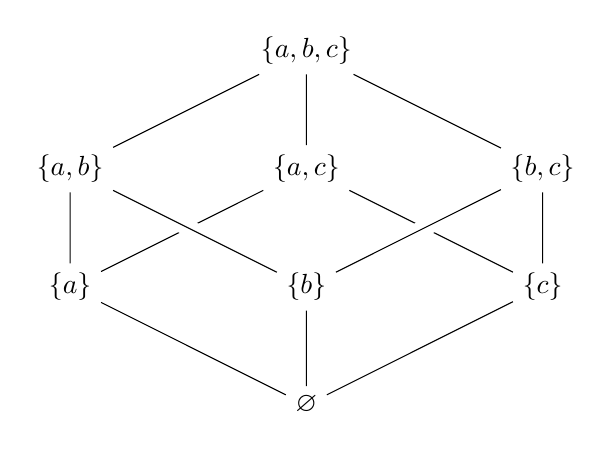
\begin{tikzpicture}
        \node (max) at (0,3) {$\{a, b, c\}$};
        \node (a) at (-3,1.5) {$\{a, b\}$};
        \node (b) at (0,1.5) {$\{a, c\}$};
        \node (c) at (3,1.5) {$\{b, c\}$};
        \node (d) at (-3,0) {$\{a\}$};
        \node (e) at (0,0) {$\{b\}$};
        \node (f) at (3,0) {$\{c\}$};
        \node (min) at (0,-1.5) {$\varnothing$};
        \draw (min) -- (d) -- (a) -- (max) -- (b) -- (f)
        (e) -- (min) -- (f) -- (c) -- (max)
        (d) -- (b);
        \draw[preaction={draw=white, -,line width=6pt}] (a) -- (e) -- (c);
    \end{tikzpicture}
\end{center}

\subsection{극대 원소와 극소 원소}
부분 순서 집합 $(A, \lesssim)$가 있을 때
\begin{itemize}
    \item 극대 원소\textsuperscript{Maximal Element}: $A$의 원소 $a$에 대하여 $a \lesssim b$인 원소 $b$가 $A$에 존재하지 않을 때 원소 $a$, 위의 하세 도표에서 $\{a, b, c\}$에 해당
    \item 극소 원소\textsuperscript{Minimal Element}: $b \lesssim a$인 원소 $b$가 $A$에 존재하지 않을 때 원소 $a$, 위의 하세 도표에서 $\varnothing$에 해당
\end{itemize}

\subsection{최대/최소 원소}
최대 원소\textsuperscript{Greatest Element}: 어떤 $a \in X$가 $X$의 모든 원소 $x$에 대해 $x \lesssim a$이면, $a$를 $X$의 최대 원소\\
최소 원소\textsuperscript{Least Element}: 어떤 $a \in X$가 $X$의 모든 원소 $x$에 대해 $a \lesssim x$이면, $a$를 $X$의 최소 원소

\newpage
\subsection{함수\textsuperscript{Function}: $f: A \to B$}
집합 $A, B$에 대해 집합 $A$에서 $B$로 가는 관계가 성립할 때,
$a \in A$에 대해 $b \in B$ 하나가 대응되는 관계\\
$$a \in A, b \in B, (a, b) \in f \text{일 때, } f(a) = b$$
대응\textsuperscript{Correspondence}:
집합 $A, B$가 있을 때, $a \in A$에 $b \in B$가 확정되는 경우 `$b$는 $a$에 대응'
\\\\
$f: A \to B$에서:
\begin{itemize}
    \item 정의역\textsuperscript{Domain}: $\mathrm{dom}(f) = A$
    \item 공변역\textsuperscript{Codomain}: $\mathrm{codom}(f) = B$
    \item 상\textsuperscript{Image}: 함수값, $f(a) = b$
    \item 치역\textsuperscript{Range}: 상의 집합, $\mathrm{ran}(f) = \{f(a)|a \in A\}$
\end{itemize}

\subsection{함수 vs 관계}
\begin{itemize}
    \item 관계
          \begin{itemize}
              \item B의 원소와 대응하지 않는 A의 원소 존재 가능
              \item 하나의 A의 원소가 하나 이상의 B의 원소와 대응 가능
          \end{itemize}
    \item 함수
          \begin{itemize}
              \item A의 모든 원소는 B의 원소와 무조건 대응
              \item 하나의 A의 원소가 하나의 B의 원소와 대응
              \item 하나의 B의 원소가 하나 이상의 A의 원소와 대응 가능
          \end{itemize}
\end{itemize}

\subsection{단사 함수\textsuperscript{Injective Function}}
\begin{itemize}
    \item 정의역 $A$의 모든 원소들이 공변역 $B$의 서로 다른 원소와 대응
    \item 일대일 함수\textsuperscript{One-to-one Function}
    \item $a_i, a_j \in A$에 대하여 $a_i \neq a_j$이면 $f(a_i) \neq f(a_j)$ 성립
    \item 단사 함수에서 함수의 치역은 공변역의 부분 집합
    \item $f:A \to B$에서 $\mathrm{ran}(f) \subseteq B$
\end{itemize}\phantom{}\\
단조 증가 함수\textsuperscript{Strictly Increasing Function}:
$x, y \in A, x < y \to f(x) < f(y)$\\\\
단조 감소 함수\textsuperscript{Strictly Decresaing Function}:
$x, y \in A, x < y \to f(x) > f(y)$\\\\
c.f.) 단조 증가 함수와 단조 감소 함수는 단사 함수
\\\\
특성: $B$의 모든 원소가 $A$의 원소와 반드시 대응하는 것은 아니므로, $|A| \leq |B|$ 성립

\newpage
\subsection{전사 함수\textsuperscript{Surjective Function}}
\begin{itemize}
    \item 공변역 $B$의 모든 원소가 정의역예 대응
    \item 치역 = 공변역, $\mathrm{ran}(f) = B$
    \item 모든 함수의 관계가 $B$의 모든 원소에 반영되므로 반영 함수\textsuperscript{Onto Function}
\end{itemize}
특성: $B$의 모든 원소가 $A$의 원소와 대응되어야 하므로 $|A| \geq |B|$ 성립

\subsection{전단사 함수\textsuperscript{Bijective Function}}
\begin{itemize}
    \item 집합 $A$의 모든 원소들이 집합 $B$의 모든 원소와 하나씩 대응
    \item 일대일 대응 함수\textsuperscript{One-to-one Correspondence Function}
\end{itemize}
특성: $A$의 모든 원소가 $B$의 모든 원소와 하나씩 일대일 대응되므로 $|A| = |B|$

\subsection{합성 함수\textsuperscript{Composition Function}}
$\forall a \in A, (g \circ f)(a) = g(f(a))$\\
결합 법칙 성립: $h\circ(g\circ f) = (h \circ g)\circ f$\\
교환 법칙 성립 X\\
특징:
\begin{itemize}
    \item $f:A \to B,\ g: B \to C$에 대해 $g \circ f$가 합성함수일 때
    \item $f$와 $g$가 단사 함수면, $g\circ f$도 단사 함수다
    \item $f$와 $g$가 전사 함수면, $g\circ f$도 전사 함수다
    \item $f$와 $g$가 전단사 함수면, $g\circ f$도 전단사 함수다
    \item $g\circ f$가 단사 함수면, $f$도 단사함수다
    \item $g\circ f$가 전사 함수면, $g$도 단사함수다
    \item $g\circ f$가 전단사 함수면, $f$는 단사함수고 $g$는 단사함수다
\end{itemize}

\subsection{항등 함수\textsuperscript{Identity Function}}
$f(a) = a$\\
전단사 함수\\
함수 $f: A \to B$고, 집합 $A$에 대한 항등 함수가 $I_A$, 집합 $B$에 대한 항등 함수가 $I_B$일 때,
$f \circ I_A = I_B \circ f = f$

\subsection{역함수\textsuperscript{Inverse Function}}
$\forall a \in A, \forall b \in B, f(a)=b \Rightarrow f^{-1}(b) = a$\\
전단사 함수일 때만 역함수 존재

\subsection{항등 함수와 역함수}
전단사 함수 $f: A \to B,\ g: B \to C$에 대해, 다음이 성립
\begin{itemize}
    \item $f^{-1} \circ f = I_A$
    \item $f \circ f^{-1} = I_B$
    \item $(g \circ f)^{-1} = f^{-1} \circ g^{-1}$
\end{itemize}

\subsection{상수 함수\textsuperscript{Constant Function}}
$\forall a \in A, \exists b \in B, f(a) = b$

\subsection{특성 함수\textsuperscript{Characteristic Function}}
$f_A(x) = \begin{cases}
        0,\quad x \not\in A \\
        1,\quad x \in A
    \end{cases}$

\subsection{올림 함수\textsuperscript{Ceiling Function}, 내림 함수\textsuperscript{Floor Function}}
올림 함수, 천정 함수 / 최소 정수 함수\textsuperscript{Least Integer Function}:
$\left\lceil x \right\rceil = n \Leftrightarrow n - 1 < x \leq n$\\
내림 함수, 바닥 함수 / 최대 정수 함수\textsuperscript{Greatest Integer Function}:
$\left\lfloor x \right\rfloor = n \Leftrightarrow n \leq x < n + 1$
\newpage
\section{Week 11}
\subsection{그래프\textsuperscript{Graph}}
공집합이 아닌 정점\textsuperscript{Vertex or Node}의 집합 $V$와 서로 다른 정점의 쌍 $(v_i, v_j)$를 연결하는 변 또는 연결선\textsuperscript{Edge}의 집합 $E$로 구성되는 구조 $G$

$G = (V, E)$

$V = \{v_1, v_2, \cdots, v_n\}$

$E = \{e_1, e_2, \cdots, e_m\} = \{(v_i, v_j), \cdots\}$\\

e.g.)
\begin{center}
    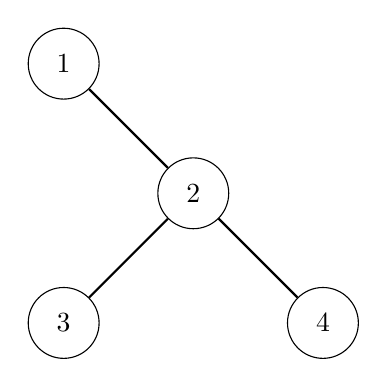
\begin{tikzpicture}
        \node[circle,draw,minimum size=0.9cm,inner sep=0pt](1){$1$};
        \node[circle,draw,minimum size=0.9cm,inner sep=0pt](2)[below right = 1cm and 1cm of 1]{$2$};
        \node[circle,draw,minimum size=0.9cm,inner sep=0pt](3)[below left = 1cm and 1cm of 2]{$3$};
        \node[circle,draw,minimum size=0.9cm,inner sep=0pt](4)[below right = 1cm and 1cm of 2]{$4$};

        \path[draw, thick]
        (1) edge node {} (2)
        (2) edge node {} (3)
        (2) edge node {} (4);
    \end{tikzpicture}
\end{center}
$$V=\{1, 2, 3, 4\},\ E=\{(1, 2), (2, 3), (2, 4)\}$$\\
무방향 그래프\textsuperscript{Undirected Graph}: 특별한 언급 없으면 무방향 그래프\\
방향 그래프\textsuperscript{Directed Graph, Digraph}: 선행자 $\to$ 후속자\\
단순 그래프\textsuperscript{Simple Graph}: 루프가 없는 그래프\\
멀티 그래프\textsuperscript{Multigraph}:
\begin{center}
    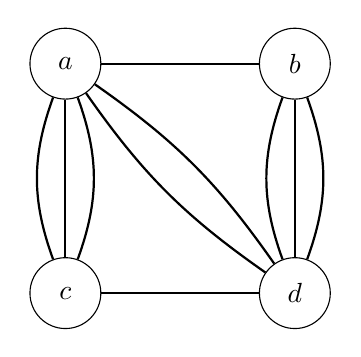
\begin{tikzpicture}
        \node[circle,draw,minimum size=0.9cm,inner sep=0pt](a){$a$};
        \node[circle,draw,minimum size=0.9cm,inner sep=0pt](b)[right = 2cm of a]{$b$};
        \node[circle,draw,minimum size=0.9cm,inner sep=0pt](c)[below = 2cm of a]{$c$};
        \node[circle,draw,minimum size=0.9cm,inner sep=0pt](d)[below = 2cm of b]{$d$};

        \path[draw, thick]
        (a) edge node {} (b)
        (a) edge[bend left = 20] node {} (c)
        (a) edge node {} (c)
        (a) edge[bend right = 20] node {} (c)
        (a) edge[bend left = 10] node {} (d)
        (a) edge[bend right = 10] node {} (d)
        (b) edge node {} (d)
        (b) edge[bend right = 20] node {} (d)
        (b) edge[bend left = 20] node {} (d)
        (c) edge node {} (d)
        ;
    \end{tikzpicture}
\end{center}
연결 그래프\textsuperscript{Connected Graph}: 모든 Vertex가 연결된 그래프, 모든 Vertex간 경로 존재\\
강한 연결 그래프\textsuperscript{Strongly Connected Graph}: 방향 그래프에서만, 모든 두 Vertex $v_1, v_2$에 대해 $v_1 \leftrightarrow v_2$\\
연결 요소\textsuperscript{Connectivity Component}: 그래프에서 모든 Vertex들이 연결되어 있는 부분 그래프

연결 수\textsuperscript{Connectivity Number}: $G$에서 연결 요소 개수
\newpage
\subsection{그래프 용어}
인접\textsuperscript{Adjacent}과 근접\textsuperscript{Incident}:\\
\begin{center}
    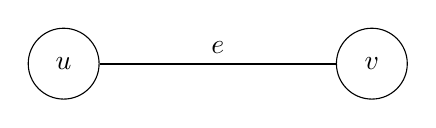
\begin{tikzpicture}
        \node[circle,draw,minimum size=0.9cm,inner sep=0pt](v){$u$};
        \node[circle,draw,minimum size=0.9cm,inner sep=0pt](u)[right = 3cm of v]{$v$};

        \path[draw, thick] (v) edge node[above] {$e$} (u);
    \end{tikzpicture}\\
    $u, v$는 서로 Adjacent, $e$는 $u, v$에 Incident
\end{center}\phantom{}
\\
루프\textsuperscript{Loop}:\\
\begin{center}
    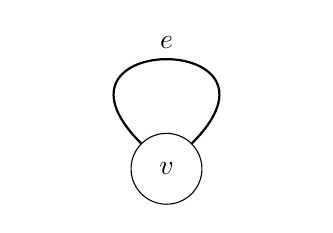
\begin{tikzpicture}
        \tikzset{every loop/.style={}}
        \node[circle,draw,minimum size=0.9cm,inner sep=0pt](v){$v$};
        \path[draw, thick] (v) edge[loop] node[above] {$e$} ();
    \end{tikzpicture}\\
    근접하는 점이 같은 $e$
\end{center}\phantom{}
\\
경로\textsuperscript{Path}: Vertex들의 열\textsuperscript{Sequence} $v_1, v_2, \cdots, v_n$에서 $(v_{k-1}, v_k) \in E, 1 \leq k < n$, 경로의 길이는 $k - 1$

단순 경로\textsuperscript{Simple Path}: 같은 Edge를 두 번 포함하지 않는 경로

기본 경로\textsuperscript{Elementary Path}: 같은 Node를 두 번 포함하지 않는 경로
\\\\
사이클\textsuperscript{Cycle} 또는 순회\textsuperscript{Circuit}: $v_1=v_k(k \neq 1)$인 경로, 종점 == 시점

단순 사이클\textsuperscript{Simple Cycle}: 같은 Edge를 반복해 방문하지 않는 사이클

기본 사이클\textsuperscript{Elementary Cycle}: 시점 제외 어떤 Node도 반복해 방문하지 않는 사이클
\\\\
길이\textsuperscript{Length}: 경로 또는 사이클을 구성하는 Edge의 수
\\\\
차수\textsuperscript{Degree} $d(v)$: Vertex $v$에 근접하는 Edge의 수, Loop는 두 개로 Count

홀수점\textsuperscript{Odd Vertex}: 차수가 홀수인 Vertex

짝수점\textsuperscript{Even Vertex}: 차수가 짝수인 Vertex
\\\\
외차수\textsuperscript{Out-degree} $\mathrm{out-}d(v)$: 방향 그래프에서 Vertex $v$에서 시작하는 화살표 수
\\\\
내차수\textsuperscript{In-degree} $\mathrm{in-}d(v)$: 방향 그래프에서 Vertex $v$에서 끝나는 화살표 수
\\\\\phantom{}
[정리] 차수에 대한 정리
\begin{itemize}
    \item $G = (V, E)$에서, 모든 Vertex의 차수의 합은 Edge의 수의 두 배

          $$\sum_{v \in V} d(v) = 2|E|$$
    \item $G = (V, E)$에서, 차수가 홀수인 정점의 수는 짝수
\end{itemize}

\newpage
\subsection{오일러 경로\textsuperscript{Eulerian Path} 및 오일러 회로\textsuperscript{Eulerian Circuit}}
오일러 경로: 멀티 그래프에서 모든 Edge들을 한 번씩만 통과하는 경로를 찾는 문제\\
오일러 회로: Node는 여러 번 통과할 수 있지만, Edge는 한 번씩만 통과하는 사이클\\\\
어떤 그래프 $G$가 오일러 경로를 가지기 위한 필요충분조건은 $G$가 연결 그래프이고, 홀수 차수의 개수가 $0$ 또는 $2$인 경우이다.\\\\
어떤 그래프 $G$가 오일러 회로를 가지기 위한 필요충분조건은 $G$가 연결 그래프이고, 모든 Node들이 짝수 개의 차수를 가지는 경우이다.

\subsection{해밀턴 경로\textsuperscript{Hamiltonian Path} 및 해밀턴 회로\textsuperscript{Hamiltonian Circuit}}
해밀턴 경로: 그래프에서 모든 Node를 오직 한 번씩만 지나지만 시점으로 돌아오지 않는 경로\\
해밀턴 회로: 그래프에서 모든 Node를 오직 한 번씩만 지나는 순회\\
해밀턴 회로에 대한 충분 조건:
\begin{itemize}
    \item 차수 1을 갖는 Node를 가진 그래프는 해밀턴 순환을 가질 수 없다.
    \item 차수가 2인 Node에 근접하는 두 Vertex는 해밀턴 순환에 포함된다.
    \item 한 Node에 근접하는 두 Vertex가 해밀턴 순환에 포함되면, 그 Node에 근접한 다른 Vertex는 해밀턴 순환에 포함될 수 없다.
\end{itemize}\phantom{}\\
Ore's Theorem: $n \geq 3$일 때, $n$개의 Node를 갖는 단순 연결 그래프 $G$에서 인접하지 않은 임의의 정점 $u, v$에 대해 $d(u) + d(v) \geq n$이면 $G$는 해밀턴 그래프이다.\\\\
Dirac's Theorem: $n \geq 3$일 때, $n$개의 Node를 갖는 단순 연결 그래프 $G$에서 임의의 정점 $v$에 대해 $2d(v) \geq n$이면 $G$는 해밀턴 그래프이다.
\newpage
\subsection{특수 형태의 그래프}
가중 그래프\textsuperscript{Weight Graph}: $G$의 각 Edge에 $0$보다 큰 수가 할당되었을 때, 이 값을 가중값\textsuperscript{Weight}이라고 하며, 이를 가중 그래프라고 한다.
\begin{center}
    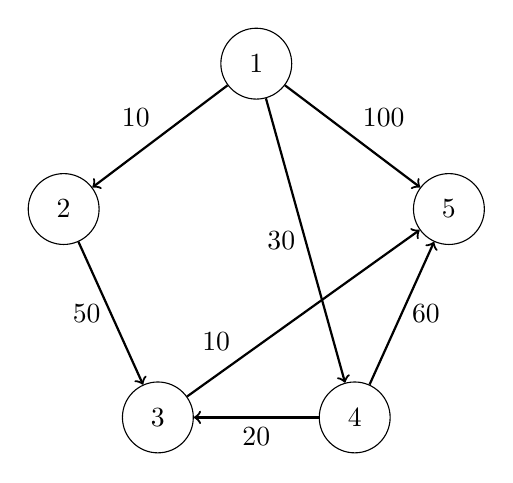
\begin{tikzpicture}
        \node[circle,draw,minimum size=0.9cm,inner sep=0pt](1){$1$};
        \node[circle,draw,minimum size=0.9cm,inner sep=0pt](2)[below left = 1.2cm and 1.8cm of 1]{$2$};
        \node[circle,draw,minimum size=0.9cm,inner sep=0pt](3)[below right = 2cm and .55cm of 2]{$3$};
        \node[circle,draw,minimum size=0.9cm,inner sep=0pt](5)[below right = 1.2cm and 1.8cm of 1]{$5$};
        \node[circle,draw,minimum size=0.9cm,inner sep=0pt](4)[below left = 2cm and .55cm of 5]{$4$};

        \path[->, draw, thick]
        (1) edge node[above left] {$10$} (2)
        (1) edge node[above right] {$100$} (5)
        (1) edge node[left] {$30$} (4)
        (2) edge node[left] {$50$} (3)
        (3) edge node[above left = -0.6cm and 0.8cm] {$10$} (5)
        (4) edge node[below] {$20$} (3)
        (4) edge node[right] {$60$} (5);
    \end{tikzpicture}
\end{center}\phantom{}\\\\
동형 그래프\textsuperscript{Isomorphic Graph}: $G_1=(V_1, E_1)$과 $G_2=(V_2, E_2)$가 주어졌을 때, 전단사 함수 $f:V_1\to V_2$가 존재하여 $\{u, v\} \in E_1 \Leftrightarrow \{f(u), f(v)\} \in E_2$이면 $f$를 동형\textsuperscript{Isomorphism}이라고 하고, $G_1$과 $G_2$를 동형 그래프라 한다.
\begin{center}
    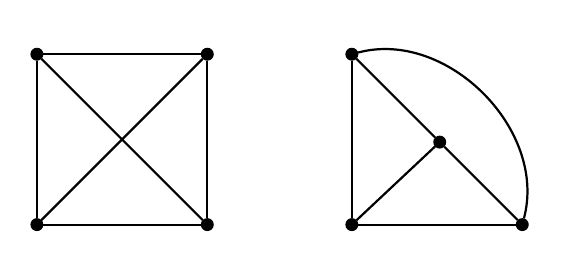
\begin{tikzpicture}
        \node[circle, fill=black, draw, minimum size=0.15cm,inner sep=0pt](1){};
        \node[circle, fill=black, draw, minimum size=0.15cm,inner sep=0pt](2)[right = 2cm of 1]{};
        \node[circle, fill=black, draw, minimum size=0.15cm,inner sep=0pt](3)[below = 2cm of 1]{};
        \node[circle, fill=black, draw, minimum size=0.15cm,inner sep=0pt](4)[below = 2cm of 2]{};

        \path[draw, thick]
        (1) edge node {} (2)
        (1) edge node {} (3)
        (1) edge node {} (4)
        (2) edge node {} (3)
        (2) edge node {} (4)
        (3) edge node {} (4);

        \begin{scope}[xshift=4cm]
            \node[circle, fill=black, draw, minimum size=0.15cm,inner sep=0pt](1){};
            \node[circle, fill=black, draw, minimum size=0.15cm,inner sep=0pt](2)[below right = 1cm and 1cm of 1]{};
            \node[circle, fill=black, draw, minimum size=0.15cm,inner sep=0pt](3)[below = 2cm of 1]{};
            \node[circle, fill=black, draw, minimum size=0.15cm,inner sep=0pt](4)[right = 2cm of 3]{};

            \path[draw, thick]
            (1) edge node {} (2)
            (1) edge node {} (3)
            (1) edge[bend left=60] node {} (4)
            (2) edge node {} (3)
            (2) edge node {} (4)
            (3) edge node {} (4);
        \end{scope}
    \end{tikzpicture}
\end{center}\phantom{}\\\\

\subsection{오일러의 정리}
연결된 평면 그래프 $G$에서 Vertex의 수를 $v$, Edge의 수를 $e$, 면\textsuperscript{Space}의 수를 $s$라고 할 때, $v - e + s = 2$
\newpage
\subsection{평면 그래프}
평면 그래프\textsuperscript{Planar Graph}: $G = (V, E)$를 평면에 그릴 때, 교차하지 않는 그래프\\
면 $f$의 차수 $d(f)$: 평면 그래프의 면 $f$의 경계를 이루는 변의 수\\
e.g.)\\
\begin{center}
    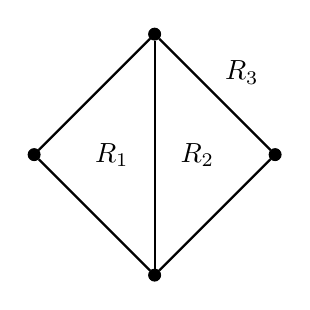
\begin{tikzpicture}
        \node[circle, fill=black, draw, minimum size=0.15cm,inner sep=0pt](1){};
        \node[circle, fill=black, draw, minimum size=0.15cm,inner sep=0pt](2)[below right = 2cm of 1]{};
        \node[circle, fill=black, draw, minimum size=0.15cm,inner sep=0pt](3)[below left = 2cm of 1]{};
        \node[circle, fill=black, draw, minimum size=0.15cm,inner sep=0pt](4)[below left = 2cm of 2]{};

        \path[draw, thick]
        (1) edge node[above right] {$R_3$} (2)
        (1) edge node {} (3)
        (1) edge node[left = .2cm] {$R_1$} (4)
        (1) edge node[right = .2cm] {$R_2$} (4)
        (2) edge node {} (4)
        (3) edge node {} (4);
    \end{tikzpicture}\\
    $d(R_1) = 3,\ d(R_2) = 3,\ d(R_3) = 4$\\
    $d(R_1)+d(R_2)+d(R_3)=2e$\\\phantom{}\\\phantom{}\\
    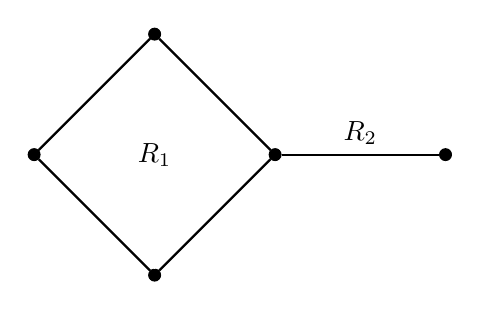
\begin{tikzpicture}
        \node[circle, fill=black, draw, minimum size=0.15cm,inner sep=0pt](1){};
        \node[circle, fill=black, draw, minimum size=0.15cm,inner sep=0pt](2)[below right = 2cm of 1]{};
        \node[circle, fill=black, draw, minimum size=0.15cm,inner sep=0pt](3)[below left = 2cm of 1]{};
        \node[circle, fill=black, draw, minimum size=0.15cm,inner sep=0pt](4)[below left = 2cm of 2]{};
        \node[circle, fill=black, draw, minimum size=0.15cm,inner sep=0pt](5)[right = 2cm of 2]{};

        \path[draw, thick]
        (1) edge node {} (2)
        (1) edge node {} (3)
        (2) edge node {} (4)
        (3) edge node {} (4)
        (2) edge node[above] {$R_2$} (5);

        \path[draw=white] (1) edge node {$R_1$} (4);
    \end{tikzpicture}\\
    $d(R_1) = 4,\ d(R_2) = 6$\\
    $d(R_1)+d(R_2)=2e$
\end{center}\phantom{}\\\\
평면 그래프의 면의 차수의 총 합은 변의 수의 두 배이다.
$$2e = \sum_{f=1}^{n} d(f)$$\\
연결된 평면 단순 그래프의 Vertex의 수를 $v$, Edge의 수를 $e$라 할 때, $v \geq 3$이면 $e \leq 3(v-2)$\\
모든 면의 차수는 3이상이므로, $2e = \sum_{f=1}^{n} d(f) \geq 3f,\ 2 = v - e + f \leq c - e + \frac{2}{3}e \leq v - \frac{1}{3}e$
\newpage
\section{Week 12}
\subsection{특수 형태의 그래프}
완전 그래프\textsuperscript{Complete Graph}: 모든 $n$개의 Vertex들의 쌍 사이에 Edge가 존재하는 $G = K_n$

e.g.)
\begin{figure}[H]
    \centering
    \begin{subfigure}[b]{0.3\textwidth}
        \centering
        
\begin{tikzpicture}
            \graph[circular placement, radius=1.8cm,
                empty nodes, nodes={circle, fill=black, draw, minimum size=0.15cm,inner sep=0pt}] {
                \foreach \x in {a} {
                        \foreach \y in {\x} {
                                \x -- \y;
                            };
                    };
            };
        \end{tikzpicture}
        \caption{$K_1$}
    \end{subfigure}
    \hfill
    \begin{subfigure}[b]{0.3\textwidth}
        \centering
        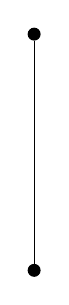
\begin{tikzpicture}
            \graph[circular placement, radius=1.5cm, group polar shift=(360/2:0),
                empty nodes, nodes={circle, fill=black, draw, minimum size=0.15cm,inner sep=0pt}] {
                \foreach \x in {a,...,b} {
                        \foreach \y in {\x,...,b} {
                                \x -- \y;
                            };
                    };
            };
        \end{tikzpicture}
        \caption{$K_2$}
    \end{subfigure}
    \hfill
    \begin{subfigure}[b]{0.3\textwidth}
        \centering
        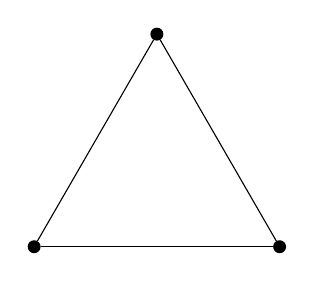
\begin{tikzpicture}
            \graph[circular placement, radius=1.8cm, group polar shift=(360/3:0),
                empty nodes, nodes={circle, fill=black, draw, minimum size=0.15cm,inner sep=0pt}] {
                \foreach \x in {a,...,c} {
                        \foreach \y in {\x,...,c} {
                                \x -- \y;
                            };
                    };
            };
        \end{tikzpicture}
        \caption{$K_3$}
    \end{subfigure}
    \begin{subfigure}[b]{0.3\textwidth}
        \centering
        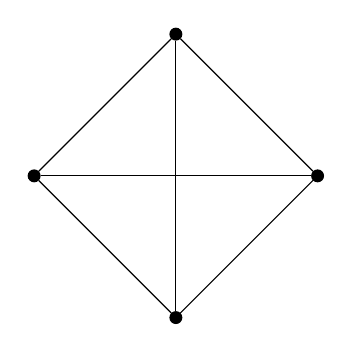
\begin{tikzpicture}
            \graph[circular placement, radius=1.8cm, group polar shift=(360/4:0),
                empty nodes, nodes={circle, fill=black, draw, minimum size=0.15cm,inner sep=0pt}] {
                \foreach \x in {a,...,d} {
                        \foreach \y in {\x,...,d} {
                                \x -- \y;
                            };
                    };
            };
        \end{tikzpicture}
        \caption{$K_4$}
    \end{subfigure}
    \hfill
    \begin{subfigure}[b]{0.3\textwidth}
        \centering
        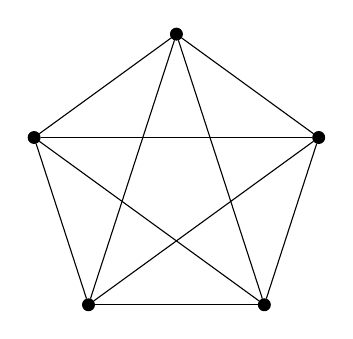
\begin{tikzpicture}
            \graph[circular placement, radius=1.9cm, group polar shift=(360/5:0),
                empty nodes, nodes={circle, fill=black, draw, minimum size=0.15cm,inner sep=0pt}] {
                \foreach \x in {a,...,e} {
                        \foreach \y in {\x,...,e} {
                                \x -- \y;
                            };
                    };
            };
        \end{tikzpicture}
        \caption{$K_5$}
    \end{subfigure}
    \hfill
    \begin{subfigure}[b]{0.3\textwidth}
        \centering
        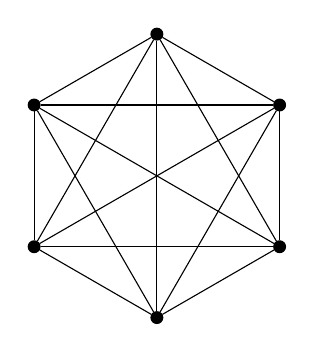
\begin{tikzpicture}
            \graph[circular placement, radius=1.8cm,
                empty nodes, nodes={circle, fill=black, draw, minimum size=0.15cm,inner sep=0pt}] {
                \foreach \x in {a,...,f} {
                        \foreach \y in {\x,...,f} {
                                \x -- \y;
                            };
                    };
            };
        \end{tikzpicture}
        \caption{$K_6$}
    \end{subfigure}
\end{figure}\phantom{}
\\\\
이분 그래프\textsuperscript{Bipartite Graph}: $V$가 $X$와 $Y = V - X$로 나누어져, 각 Edge가 X 내의 Vertex와 Y 내의 Vertex의 쌍으로 연결될 때, $G = (V, E)$\\
완전 이분 그래프\textsuperscript{Complete Bipartite Graph}: $X$내의 모든 Vertex와 $Y$내의 모든 Vertex 사이에 Edge가 존재할 때, 그래프 $G$

e.g.)
\begin{figure}[H]
    \centering
    \hfill
    \begin{subfigure}[b]{0.3\textwidth}
        \centering

        \tikz \graph[nodes={circle, fill=black, empty nodes, draw, minimum size=0.15cm,inner sep=0pt}] {
        {1,2} -- [complete bipartite] {a,b,c}
        };
        \caption{$K_{2, 3}$}
    \end{subfigure}
    \hfill
    \begin{subfigure}[b]{0.3\textwidth}
        \centering

        \tikz \graph[nodes={circle, fill=black, empty nodes, draw, minimum size=0.15cm,inner sep=0pt}] {
        {1,2} -- [complete bipartite] {a,b,c,d}
        };
        \caption{$K_{2, 4}$}
    \end{subfigure}
    \hfill
    \hfill
\end{figure}\phantom{}

\subsection{그래프의 표현 방법}
인접 행렬\textsuperscript{Adjacency Matrix}: $G = (V, E)$에서, $|V| = n$일 때, $G$의 인접 행렬은 $n \times n$ 행렬 $A$
$$a_{ij} = \begin{cases}
        1 \quad (v_i, v_j)\in E \\
        0 \quad \text{otherwise}
    \end{cases}$$
\\\\
인접 리스트\textsuperscript{Adjacency List}: 각 Vertex에 대해 포인터가 주어지고, 그 Vertex로 부터 인접한 Vertex들을 모두 Linked List에 담음 (List 내에서는 순서에 관계가 없음)

Linked List는 Node의 연결로 표현
\begin{itemize}
    \item Head: Linked List의 시작 Node (그래프의 각 Vertex들)
    \item Node: 데이터 필드 + 포인트 필드 (다음에 연결된 Node의 주소 저장)
    \item 마지막 Node의 포인트 필드는 \texttt{null}
\end{itemize}

\subsection{그래프의 응용 및 활용}
최단 경로 찾기\textsuperscript{Shortest Path Problem}: 다익스트라\textsuperscript{Dijkstra} 알고리즘

e.g.)
\begin{center}
    \begin{minipage}{0.48\textwidth}
        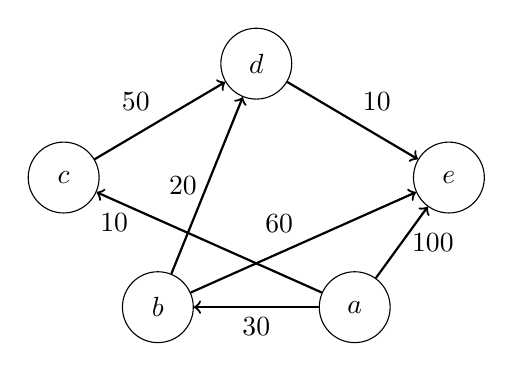
\begin{tikzpicture}
            \node[circle,draw,minimum size=0.9cm,inner sep=0pt](d){$d$};
            \node[circle,draw,minimum size=0.9cm,inner sep=0pt](c)[below left = 0.8cm and 1.8cm of d]{$c$};
            \node[circle,draw,minimum size=0.9cm,inner sep=0pt](b)[below right = 1cm and .55cm of c]{$b$};
            \node[circle,draw,minimum size=0.9cm,inner sep=0pt](e)[below right = 0.8cm and 1.8cm of d]{$e$};
            \node[circle,draw,minimum size=0.9cm,inner sep=0pt](a)[below left = 1cm and .55cm of e]{$a$};

            \path[->, draw, thick]
            (c) edge node[above left] {$50$} (d)
            (d) edge node[above right] {$10$} (e)
            (b) edge node[above left] {$60$} (e)
            (a) edge node[below] {$30$} (b)
            (a) edge node[right] {$100$} (e)
            (b) edge node[left] {$20$} (d)
            (a) edge node[below left = -0.5cm and 0.9cm] {$10$} (c);
        \end{tikzpicture}
    \end{minipage}
    \begin{minipage}{0.48\textwidth}
        \begin{equation*}
            \begin{bNiceMatrix}[first-row, first-col]
                  & a      & b      & c      & d      & e      \\
                a & 0      & 30     & 10     & \infty & 100    \\
                b & \infty & 0      & \infty & 20     & 60     \\
                c & \infty & \infty & 0      & 50     & \infty \\
                d & \infty & \infty & \infty & 0      & 10     \\
                e & \infty & \infty & \infty & \infty & 0      \\
            \end{bNiceMatrix}
        \end{equation*}
    \end{minipage}
\end{center}\phantom{}\\\\
위와 같은 그래프가 주어졌을 때,\\
\begin{center}
    \begin{tabular}[1.5]{c|c|c|c|c|c|c}
        $S$              &     & \texttt{D[a]} & \texttt{D[b]} & \texttt{D[c]} & \texttt{D[d]} & \texttt{D[e]} \\
        \hline
        $\{a\}$          & $a$ & $0$           & $30$          & $10$          & $\infty$      & $100$         \\
        $\{a, c\}$       & $c$ &               & $30$          & $10$          & $60$          & $100$         \\
        $\{a, c, b\}$    & $b$ &               & $30$          &               & $50$          & $90$          \\
        $\{a, c, b, d\}$ & $d$ &               &               &               & $50$          & $60$          \\
    \end{tabular}
\end{center}\phantom{}\\\\
해밀턴 순회의 응용: 일반적인 해결 알고리즘 존재 X $\to$ 최근접 이웃 방법\textsuperscript{Nearest Neighbour Method}(Greedy 알고리즘)
\newpage
\subsection{그래프의 탐색(Traversal)}
깊이 우선 탐색\textsuperscript{Depth First Search; DFS}: Stack or 재귀로 구현
\begin{itemize}
    \item 시작 Vertex $v$에서 인접 Vertex 중 방문하지 않은 Vertex $w$ 방문
    \item $w$에서 다시 인접 Vertex 중 방문하지 않은 Vertex $u$ 방문 반복
    \item 어떤 Vertex $\nu$ 방문 후 $\nu$에 인접한 모든 Vertex 방문한 경우, 바로 이전 Vertex로 돌아가 위 반복
    \item 모든 Vertex 방문 후 탐색 종료
\end{itemize}
\phantom{}\\
너비 우선 탐색\textsuperscript{Breadth First Search; BFS}: Queue 사용
\begin{itemize}
    \item 시작 Vertex $v$에서 인접한 Vertex 모두 차례로 방문
    \item 더 이상 방문할 Vertex가 없을 때, 다시 $v$에 인접한 Vertex중 처음 방문한 Vertex와 인접한 Vertex 방문
    \item $v$에 인접한 Vertex중 두 번째 방문한 Vertex와 인접한 Vertex 방문 반복
    \item 모든 Vertex 방문 후 탐색 종료
\end{itemize}

\subsection{트리}
트리(Tree):
\begin{itemize}
    \item A connected undirected graph with no circuits
    \item An undirected graph is a tree iff there is a unique simple path between any two of its vertices
    \item 특별히 지정된 노드인 루트가 있고, 나머지 노드들은 다시 각각 트리이면서 연결되지 않는(disjoint) $T_1, T_2, \cdots, T_n(n \geq 0, T_n\text{은 루트의 서브 트리\textsuperscript{Subtree}})$으로 나누어 진다.
\end{itemize}\phantom{}
\\
루트\textsuperscript{Root}: 주어진 트리의 시작 노드, 트리의 가장 높은 곳에 위치\\
차수\textsuperscript{Degree}: 각 노드의 서브 트리의 개수\\
잎 노드 or 단말 노드\textsuperscript{Leaf Node}: 차수가 0인 노드\\
자식 노드\textsuperscript{Children Node}: 어떤 노드의 서브 트리의 루트 노드\\
부모 노드\textsuperscript{Parent Node}: 자식 노드의 반대\\
형제 노드\textsuperscript{Sibling Node}: 동일한 부모를 가지는 노드\\
중간 노드\textsuperscript{Internal Node}: 자식 노드를 갖는 노드\\
조상\textsuperscript{Ancestor}: 루트로부터 각 노드에 이르는 경로 상에 나타난 모든 노드들\\
자손\textsuperscript{Descendant}: 각 노드부터 잎 노드에 이르는 경로 상에 나타난 모든 노드들\\
레벨\textsuperscript{Level}: 루트의 레벨 $= 0$, 자손 노드로 내려가며 \texttt{++}\\
트리의 높이 or 깊이\textsuperscript{Height or Depth}: 트리에서 노드가 가질 수 있는 맥스 레벨\\
숲\textsuperscript{Forest}: 서로 연결되지 않는 트리들의 집합, 트리에서 루트를 제거 $\to$ 숲 생성
\\\\
$G$는 트리\\
$\equiv$ $G$는 연결되어 있고, $M = n - 1$\\
$\equiv$ $G$는 연결되어 있고, 어느 한 연결선만을 제거하더라도 $G$는 연결되지 않음\\
$\equiv$ $G$는 사이클을 가지지 않고, $m = n - 1$\\
$\equiv$ $G$는 어느 한 연결선만 첨가하더라도 사이클 형성\\

\subsection{이진 트리}
이진 트리\textsuperscript{Binary Tree}: 노드들의 유한 집합, 공집합이거나, 루트와 왼쪽 서브 트리, 오른쪽 서브 트리로 이루어짐\\
사향 이진 트리\textsuperscript{Skewed Binary Tree}: 왼쪽 or 오른쪽으로 편향된 트리\\
완전 이진 트리\textsuperscript{Complete Binary Tree}: 높이가 $k$일 때 레벨 $1$부터 $k-1$까지는 모두 차있고 레벨 $k$에서는 왼쪽 노드부터 차례로 차있는 이진 트리\\
포화 이진 트리\textsuperscript{Full Binary Tree}: 잎 노드가 아닌 것들은 모두 $2$개씩 자식 노드를 가지며 트리의 높이가 일정할 때
\\\\
완전 $n$-ary 트리: 레벨이 $k$일 때, 레벨 $1$부터 $k-1$까지는 모두 n개의 자식 노드를 가지고, 레벨 $k$에서는 왼쪽 노드부터 차례로 차있는 트리\\
포화 $n$-ary 트리: 모든 중간 노드가 $n$개의 자식 노드를 가지는 트리

포화 $n$-ary 트리에서 $m$개의 중간 노드를 가질 때, 전체 노드 개수 $= (m + 1) * n + 1$(루트 노드)
\\\\
이진 트리가 레벨 $i$에서 가질 수 있는 최대 노드 수 $= 2^i$\\
높이가 $k$인 이진 트리가 가질 수 있는 최대 전체 노드 수 $= 2^{k + 1} - 1$\\
잎 노드 개수 $= n_0$, 차수가 $2$인 노드 개수 $= n_2$일 때, $n_0 = n_2 + 1$ 항상 성립

\subsection{이진 트리의 표현}
배열:
\begin{itemize}
    \item 트리의 중간에 새로운 노드를 삽입하거나 기존의 노드를 지울 때 비효율적
    \item 높이가 $h$인 이진 트리는 각 노드 번호를 인덱스로 하여 1차원 배열로 구현 가능 (인덱스는 1부터 시작)
    \item 노드 인덱스 $n$의 부모 인덱스 $= \left\lfloor \dfrac{n}{2} \right\rfloor$
    \item 노드 인덱스 $n$의 왼쪽 자식 인덱스 $= 2n$, 오른쪽 자식 인덱스 $= 2n + 1$
\end{itemize}\phantom{}\\
연결 리스트: 일반적으로 가장 많이 사용. 중간 데이터, 왼쪽 자식 포인터, 오른쪽 자식 포인터 저장

\newpage
\section{Week 13}
\subsection{이진 트리의 탐방}
트리의 각 노드를 꼭 한 번씩만 방문\textsuperscript{Traversal}하는 방법
\begin{itemize}
    \item 각 노드와 그 노드의 서브 트리를 같은 방법으로 탐방
    \item 전순위, 중순위, 후순위 탐방 기법
    \item D: 노드, L: 노드의 왼쪽 서브 트리, R:노드의 오른쪽 서브 트리
    \item 왼쪽을 오른쪽보다 항상 먼저 방문한다고 가정
    \item 중순위: LDR
    \item 전순위: DLR
    \item 후순위: LRD
    \item 수식 표현에서 중순위 표기\textsuperscript{Infix}, 전순위 표기\textsuperscript{Prefix}, 후순위 표기\textsuperscript{Postfix}와 각각 대응
\end{itemize}\phantom{}\\
탐방의 결과, 각 노드에 들어있는 데이터를 차례로 나열\\\\
중순위:
\begin{minted}[linenos, fontsize=\small, breaklines]{cpp}
void inOrder(TREE* currentNode) {
    if (currentNode != NULL) {
        inOrder(currentNode->leftChild);
        std::cout << currentNode->data;
        inOrder(currentNode->rightChild);
    }
}
\end{minted}
전순위:
\begin{minted}[linenos, fontsize=\small, breaklines]{cpp}
void preOrder(TREE* currentNode) {
    if (currentNode != NULL) {
        std::cout << currentNode->data;
        preOrder(currentNode->leftChild);
        preOrder(currentNode->rightChild);
    }
}
\end{minted}
후순위:
\begin{minted}[linenos, fontsize=\small, breaklines]{cpp}
void postOrder(TREE* currentNode) {
    if (currentNode != NULL) {
        postOrder(currentNode->leftChild);
        postOrder(currentNode->rightChild);
        std::cout << currentNode->data;
    }
}
\end{minted}

\subsection{순회 표기 \& 수식 트리}
중순위: $(a+b)\times(c-d)$\\
전순위: $\times + ab-cd$\\
후순위: $ab+cd-\times$\\\\
전순위 수식 $+-\times\ 2\ 3\ 5 \div \wedge\  2\ 3\ 4$ \texttt{==} 중순위 수식 $2 \times 3 - 5 + 2^3 \div 4$\\
후순위 수식 $7\ 2\ 3\times - 4 \wedge 9\ 3 \div +$ \texttt{==} 중순위 수식 $(7 - 2 \times 3)^4 + 9 \div 3$
\\\\
후순위 표기식과 스택을 활용하여 수식 트리 생성:

후순위 표기식이 주어지면 스택에 피연산자 저장

연산자를 만나면 스택에서 두 개의 피연산자 \texttt{pop()} 후 연산 결과(트리) 다시 저장

\subsection{생성 트리와 최소 비용 생성 트리}
생성 트리\textsuperscript{Spanning Tree}: $\exists G$에서 모든 노드들을 포함하는 트리

비용\textsuperscript{Cost}: 트리 연결선의 값의 합\\
최소 비용 생성 트리(Minimum Spanning Tree: MST): 생성 트리 중 최소 비용
\\\\
Prim's Algorithm:
\begin{itemize}
    \item $G = (V, E)$에서 $V = \{1, 2, \cdots, n\}$
    \item 노드의 집합 $U$를 $1$로 시작
    \item $u \in U,\ v \in V - U$일 때, $U$와 $V-U$를 연결하는 사이클 형성 X인 가장 짧은 연결선 $(u, v)$를 찾아 $v$를 $U$에 포함시킴
    \item 위를 $U-V$까지 반복
\end{itemize}
\begin{minted}[linenos, fontsize=\small, breaklines, escapeinside=||, mathescape=true]{cpp}
    void prim(graph G: set_of_edges T) {
        set_of_vertices U;
        vertex u, v;
        T = NULL;
        U = {1};
        while (U != V) {
            let (u, v) be a lowest cost edge such that u is in U and v is in V - U;
            if ((u, v) does not create a cycle) {
                T = T |$\cup$| {(u, v)};
                U = U |$\cup$| {v};
            }
        }
    }
\end{minted}
\phantom{}
\newpage
Kruskal Algorithm:
\begin{itemize}
    \item $G = (V, E)$에서 $V = \{1, 2, \cdots, n\}$, $T =$ (연결선의 집합)
    \item Let $T = \varnothing$
    \item $E$를 비용이 적은 순서로 정렬
    \item 가장 최솟값 가진 연결선 $(u, v)$ 차례로 찾아 사이클 형성 X이면 $T$에 포함
    \item 위를 $|T| = |V| - 1$까지 반복
\end{itemize}
\begin{minted}[linenos, fontsize=\small, breaklines, escapeinside=||, mathescape=true]{cpp}
    void kruskal(graph G: set_of_edges T) {
        T = NULL;
        while (T contains less than n - 1 edges and E is not empty) {
            choose an edge (v, w) from E of lowest cost;
            delete (v, w) from E;
            if ((v, w) does not create a cycle in T)
                add (v, w) to T;
            else discard (v, w);
        }
        if (T contains fewer than n - 1 edges)
            std::cout << "No Spanning Tree";
    }
\end{minted}

\subsection{트리의 활용}
문법의 파싱\textsuperscript{Parsing}\\
허프만 코드\textsuperscript{Huffman Code}:
\begin{itemize}
    \item 알파벳 문자를 $0$과 $1$의 비트 코드로 Encoding
    \item 문자의 발생 빈도에 따라 코드의 길이를 다르게 $\to$ 통신의 효율성
    \item 접두어 성질: 어떤 문자 코드도 다른 문자 코드의 접두어 코드가 아님
\end{itemize}\phantom{}\\
Huffman Algorithm:
\begin{itemize}
    \item 발생 빈도가 가장 낮은 두 문자를 선택해 하나의 이진 트리로 연결
          \begin{itemize}
              \item 왼쪽 노드에는 빈도수 낮은 문자, 오른쪽 노드에는 빈도수 높은 문자
              \item 그 두 문자의 루트 노드는 두 문자의 빈도의 합
              \item 문자들을 이진 트리로 연결
              \item 그 후에 이진 트리들을 연결
          \end{itemize}
    \item 위 과정을 모든 문자가 하나의 이진 트리로 묶일 때까지 반복
    \item 생성된 이진 트리의 왼쪽 노드는 $0$, 오른쪽 노드에는 $1$ 부여
    \item 루트부터 해당 문자까지 $0$ 또는 $1$을 순서대로 나열한 것이 해당 문자의 허프만 코드
\end{itemize}

\newpage
\section{Week 14}
\subsection{이진 탐색 트리}
이진 탐색 트리\textsuperscript{Binary Search Tree}:
\begin{itemize}
    \item 모든 노드 $x$에 대하여 노드 $y$가 노드 $x$의 왼쪽 서브 트리에 있을 때 $y < x$이고,
          노드 $z$가 노드 $x$의 오른쪽 서브 트리에 있으면 $x < z$인 이진 트리
    \item $<$는 순서 관계를 의미
    \item 높이 균형 이진 트리인 경우 탐색 시간은 $\log n$
\end{itemize}

\subsection{결정 트리}
결정 트리\textsuperscript{Decision Tree}: 8개의 동전 문제
\newpage
\subsection{부울식}
0과 1의 조합으로 연산\\
$A = \{0, 1\}$에 대해 이항 연산자\textsuperscript{Binary Operator} $+$\textsuperscript{OR}과 $\cdot$\textsuperscript{AND} 및
단항 연산자\textsuperscript{Unary Operator} $'$\textsuperscript{Complement}로 표현되는 식\\
연산 우선 순위: $' > \cdot > +$\\\\
두 부울식이 같은 진리표\textsuperscript{Truth Table}을 가질 때 동치\textsuperscript{Equivalent}, 연산자는 $=$

\begin{table}[h]
    \caption {부울식의 법칙}
    \centering
    \begin{tabular}[1.5]{c|c}
        이름                                         & 법칙                                                                                                                                        \\
        \Xhline{3\arrayrulewidth}
        멱등 법칙\textsuperscript{Idempotent Law}      & \begin{tabular}[1.5]{@{}c@{}}$p \cdot p = p$\\$p + p = p$\end{tabular}                                                                    \\
        \hline
        항등 법칙\textsuperscript{Identity Law}        & \begin{tabular}[1.5]{@{}c@{}}$p + 0 = p$\\$p \cdot 1 = p$\end{tabular}                                                                    \\
        \hline
        교환 법칙\textsuperscript{Commutative Law}     & \begin{tabular}[1.5]{@{}c@{}}$p + q = q + p$\\$p \cdot q = q \cdot p$\end{tabular}                                                        \\
        \hline
        결합 법칙\textsuperscript{Associative Law}     & \begin{tabular}[1.5]{@{}c@{}}$p + (q + r) = (p + q) + r$\\$p\cdot(q \cdot r) = (p \cdot q) \cdot r$\end{tabular}                          \\
        \hline
        분배 법칙\textsuperscript{Distributive Law}    & \begin{tabular}[1.5]{@{}c@{}}$p + (q \cdot r) = (p + q)\cdot(p + r)$\\$p \cdot (q + r) = (p \cdot q)+(p \cdot r)$\end{tabular} \\
        \hline
        흡수 법칙\textsuperscript{Absorption Law}      & \begin{tabular}[1.5]{@{}c@{}}$p+(p\cdot q) = p$\\$p \cdot (p + q) = p$\end{tabular}                                                       \\
        \hline
        역 법칙\textsuperscript{Inverse Law}          & \begin{tabular}[1.5]{@{}c@{}}$p + p'$\\$p\cdot p' = 0$\end{tabular}                                                                       \\
        \hline
        보 법칙\textsuperscript{Complement Law}       & $(p')' = p$                                                                                                                               \\
        \hline
        우등 법칙\textsuperscript{Dominance Law}       & \begin{tabular}[1.5]{@{}c@{}}$p + 1 = 1$\\$p \cdot 0 = 0$\end{tabular}                                                                    \\
        \hline
        드 모르간의 법칙\textsuperscript{De Morgan's law} & \begin{tabular}[1.5]{@{}c@{}}$(p + q)' = p' \cdot q'$\\$(p \cdot q)' = p' + q'$\end{tabular}
    \end{tabular}
\end{table}

\subsection{부울 함수\textsuperscript{Boolean Function}}
부울 변수와 부울 연산자로 구성된 부울식\\
$n$개의 부울 변수 $x_1, x_2, \cdots, x_n$에 대한 부울 함수는 $f(x_1, x_2, \cdots, x_n)$으로 표현\\
$n$개의 부울 변수가 있을 때, 그 변수들로부터 얻을 수 있는 조합은 $2^n$개
\\\\
리터럴\textsuperscript{Literal}: 부울 함수를 구성하는 부울 변수 또는 그의 보수\\
최소항\textsuperscript{Minterm}: $n$차 부울함수 $f(x_1, x_2, \cdots, x_n)$을 구성하는 논리곱 항들 중 $n$개의 리터럴 곱으로 구성된 항

\subsection{최소항}
부울 함수는 부울 변수에 대한 최소항들 중에서 $1$의 값을 가지는 최소항들의 부울 합을 식으로 표현하는 함수

e.g.)
\begin{center}
    \begin{tabular}[1]{c|c|c|c}
        $x$ & $y$ & $z$ & $f(x, y, z)$ \\
        \hline
        0   & 0   & 0   & 0            \\
        0   & 0   & 1   & 1            \\
        0   & 1   & 0   & 0            \\
        0   & 1   & 1   & 0            \\
        1   & 0   & 0   & 1            \\
        1   & 0   & 1   & 0            \\
        1   & 1   & 0   & 1            \\
        1   & 1   & 1   & 0
    \end{tabular}
\end{center}\phantom{}\\\\
부울 함수는 $f(x, y, z)=1$인 최소항들의 합이므로 $f(x, y, z) = x' y' z + xy' z' + xyz'$이다.

\subsection{정규식\textsuperscript{Disjunctive Normal Form; DNF}}
최소항들의 부울합으로 표현된 부울 함수\\
최소항들은 부울 변수의 곱으로 표현\\
곱의 합(Sum of Products) 또는 논리합 표준형
\\\\
정규식이 아닌 부울 함수를 정규식으로 표현하는 방법:
\begin{itemize}
    \item 진리표를 이용한 정규식 변환
    \item 부울 법칙을 이용한 정규식 변환
          \begin{itemize}
              \item 각 항에 포함되지 않은 부울 변수를 파악
              \item 각 항에 포함되지 않은 부울 변수에 대해
              \item 논리곱에 대한 항등 법칙 $x \cdot 1 = x$와
              \item 논리합에 대한 보수 법칙 $x + x' = 1$을 적용
              \item 각 항에 없는 부울 변수 추가
              \item 분배 법칙 등을 이용해 식을 풀고, 중복되는 항은 멱등 법칙에 의해 제거
          \end{itemize}
          e.g.) \begin{align*}
              f(x, y) & = x + y'                  &                         \\
                      & = x\cdot 1 + y' \cdot 1   & (\because \text{항등 법칙}) \\
                      & = x(y + y') + y' (x + x') & (\because \text{보수 법칙}) \\
                      & = xy + xy' + y'x + y'x'   & (\because \text{분배 법칙}) \\
                      & = xy + xy' + xy' + x'y'   & (\because \text{교환 법칙}) \\
                      & = xy + xy' + x'y'         & (\because \text{멱등 법칙})
          \end{align*}
          $$\therefore f(x, y) = xy + xy' + x'y'$$
\end{itemize}

\subsection{예제 풀이}
1. $(x+y)(y+z)(z+x)= xy + yz + zx$
\begin{align*}
    (x+y)(y+z)(z+x) & = (xy + xz + yy + yz)(z + x)      \\
                    & = (xy + xz + y + yz)(z + x)       \\
                    & = (xy + xz + y (1 + z))(z + x)    \\
                    & = (xy + xz + y)(z + x)            \\
                    & = xyz + xxy + xzz + xxz + yz + xy \\
                    & = xyz + xy + yz + zx              \\
                    & = xy(z + 1) + yz + zx             \\
                    & = xy + yz + zx
\end{align*}\phantom{}
\\\\
2. $xy + yz + x' z = xy + x' z$
\begin{align*}
    xy + yz + x' z & = xy + 1\cdot yz + x' z   \\
                   & = xy + (x+x')yz + x' z    \\
                   & = xy + xyz + x' yz + x' z \\
                   & = xy(1 + z) + x' z(y + 1) \\
                   & = xy + x' z
\end{align*}

\newpage
\section{Week 15}
\subsection{부울 함수의 간소화}
더 적은 변수와 연산자를 사용하여 같은 기능 또는 결과 도출\\
부울 함수를 간소화 하는 방법:
\begin{itemize}
    \item 부울식의 기본 법칙 사용 $\to$ 과정이 복잡하고 간소화에 대한 확인이 쉽지 않음
    \item 카르노맵을 사용
\end{itemize}\phantom{}
\\\\
카르노맵\textsuperscript{Karnaugh Map}:
\begin{itemize}
    \item 부울 함수가 가질 수 있는 모든 경우의 최소항들을 사각형 형태의 표에 배열한 후,
          $1$의 값을 가지는 최소항들만 $1$로 표시
          \begin{itemize}
              \item $1$을 갖는 항들을 연결하여 최소화
          \end{itemize}
    \item 사각형 내 배치 시, 인접한 최소항들은 변수 하나 차이만 있도록 배치
          \begin{itemize}
              \item $xy$와 $xy'$은 인접 가능
              \item $xy$와 $x'y'$은 인접 불가
          \end{itemize}
\end{itemize}\phantom{}\\\\
두 변수에 대한 카르노맵: 변수를 $x, y$라 할 때, 모든 가능한 최소항 조합
\begin{itemize}
    \item $x'y', x'y, xy', xy$
    \item $x$가 $0$이고, $y$가 $0$일 때, 부울식은 $x'y'$
\end{itemize}
\begin{figure}[H]
\begin{subfigure}[b]{0.45\textwidth}
\centering
\begin{karnaugh-map}[2][2][1][$y$][$x$]
\manualterms{$x'y'$, $x'y$, $xy'$, $xy$}
\end{karnaugh-map}
\caption{두 변수에 대한 카르노 맵}
\end{subfigure}
\begin{subfigure}[b]{0.45\textwidth}
\centering
\begin{karnaugh-map}[2][2][1][$y$][$x$]
\minterms{0,1,2}
% \autoterms[a]
% \implicant{1}{1}
\end{karnaugh-map}
\caption{$f(x, y) = x'y'+x'y+xy'$의 카르노 맵}
\end{subfigure}
\end{figure}
\newpage
간소화: $1$로 표시된 사각형이 인접할 경우, 함께 묶을 수 있는 경우

e.g.)
\begin{figure}[H]
\begin{subfigure}[b]{0.45\textwidth}
\centering
\begin{karnaugh-map}[2][2][1][$y$][$x$]
\minterms{0,3}
% \implicant{0}{1}
\end{karnaugh-map}
\caption{인접한 경우 없음: $x'y'+xy$}
\end{subfigure}
\hfill
\begin{subfigure}[b]{0.45\textwidth}
\centering
\begin{karnaugh-map}[2][2][1][$y$][$x$]
\minterms{0,1}
\implicant{0}{1}
\end{karnaugh-map}
\caption{$y$의 값에 관계없이 $x$의 값이 $0$: $x'$ ($x'$일 때 $1$)}
\end{subfigure}
\begin{subfigure}[b]{0.45\textwidth}
\centering
\begin{karnaugh-map}[2][2][1][$y$][$x$]
\minterms{0,1,2}
\implicant{0}{1}
\implicant{0}{2}
\end{karnaugh-map}
\caption{(b)의 경우 + $x$의 값에 관계 없이 $y'$: $x'+y'$}
\end{subfigure}
\hfill
\begin{subfigure}[b]{0.45\textwidth}
\centering
\begin{karnaugh-map}[2][2][1][$y$][$x$]
\minterms{0,1, 2, 3}
\implicant{0}{3}
\end{karnaugh-map}
\caption{$x$와 $y$의 값에 관계없이 항상 $1$: $1$}
\end{subfigure}
\end{figure}\phantom{}\\\\
세 변수에 대한 카르노 맵:
\begin{itemize}
    \item $yz$에 대한 사각형에서 $00, 01$ 다음에 $11$ (인접하는 행 또는 열에서 1비트 차이만 나야함)
    \item 왼쪽 끝은 오른쪽 끝과 인접하다 생각하기
\end{itemize}

\begin{figure}[H]
\begin{subfigure}[b]{0.45\textwidth}
\centering
\begin{karnaugh-map}[4][2][1][$z$][$y$][$x$]
\manualterms{$x'y'z'$, $x'y'z$, $x'yz'$, $x'yz$, $xy'z'$, $xy'z$, $xyz'$, $xyz$}
\end{karnaugh-map}
\caption{세 변수에 대한 카르노 맵}
\end{subfigure}
\hfill
\begin{subfigure}[b]{0.45\textwidth}
\centering
\begin{karnaugh-map}[4][2][1][$z$][$y$][$x$]
\minterms{0, 2, 4, 6}
\implicantedge{0}{4}{2}{6}
\end{karnaugh-map}
\caption{$f(x, y, z) = x'y'z'+x'yz+xy'z'+xyz = z'$}
\end{subfigure}
\end{figure}\phantom{}\\\\
네 변수에 대한 카르노 맵:
\begin{itemize}
    \item $01$ 다음 $11$
    \item 왼쪽 끝과 오른쪽 끝 인접
    \item 위쪽 끝과 아래쪽 끝 인접
\end{itemize}
\begin{figure}[H]
\begin{subfigure}[t]{0.45\textwidth}
\centering
\begin{karnaugh-map}[4][4][1][$w$][$z$][$y$][$x$]
\manualterms{
    $x'y'z'w'$, $x'y'z'w$, $x'y'zw'$, $x'y'zw$,
    $x'yz'w'$, $x'yz'w$, $x'yzw'$, $x'yzw$,
    $xy'z'w'$, $xy'z'w$, $xy'zw'$, $xy'zw$,
    $xyz'w'$, $xyz'w$, $xyzw'$, $\phantom{'}xyzw\phantom{'}$
}
\end{karnaugh-map}
\caption{네 변수에 대한 카르노 맵}
\end{subfigure}
\hfill
\begin{subfigure}[t]{0.45\textwidth}
\centering
\begin{karnaugh-map}[4][4][1][$w$][$z$][$y$][$x$]
\minterms{0, 2, 8, 10, 5, 7, 13, 15}
\implicantcorner[0]
\implicant{5}{15}
\end{karnaugh-map}
\caption{$f(x, y, z, w) = x'y'z'w'+x'y'zw'+x'yz'w+x'yzw+xyz'w+xyzw+xy'z'w'+xy'zw' = yw+y'w'$}
\end{subfigure}
\end{figure}
\newpage
\subsection{논리 회로\textsuperscript{Logic Circuit}}
\begin{itemize}
    \item 논리 회로의 입출력은 논리 게이트\textsuperscript{Gate}들을 상호 연결해 구성
    \item 입력은 부울 변수, 출력은 부울 함수, 부울 연산자는 게이트
    \item $1$ = On, $0$ = Off
\end{itemize}
\phantom{}\\
회로를 설계하기 전에 먼저 부울식을 간소화하는 과정이 필요
\\
논리 함수의 완전성\textsuperscript{Completeness}: 부울 연산자 AND, OR, NOT만으로도 모든 논리 함수들을 나타낼 수 있다.\\\\
\begin{table}[H]
    \centering
    \caption{여러 가지 논리 게이트}
    \begin{tabular}[1]{c|m{1.9cm}|c}
        게이트  & 기호                                 & 수식            \\
        \Xhline{3\arrayrulewidth}
        AND  & \begin{circuitikz} \draw
                   (0,0) node[and port] (myand1) {};
               \end{circuitikz}  & $x = A \cdot B$                \\
        \hline
        OR   & \begin{circuitikz} \draw
                   (0,0) node[or port] (myand1) {};
               \end{circuitikz}   & $x = A + B$                   \\
        \hline
        NOT  & \begin{circuitikz} \draw
                   (0,0) node[not port] (myand1) {};
               \end{circuitikz}  & $x = A'$                   \\
        \hline
        NAND & \begin{circuitikz} \draw
                   (0,0) node[nand port] (myand1) {};
               \end{circuitikz} & $x = (A \cdot B)'$              \\
        \hline
        NOR  & \begin{circuitikz} \draw
                   (0,0) node[nor port] (myand1) {};
               \end{circuitikz}  & $x = (A + B)'$                 \\
        \hline
        XOR  & \begin{circuitikz} \draw
                   (0,0) node[xor port] (myand1) {};
               \end{circuitikz}  & $x = A \oplus B = A'B+AB'$     \\
        \hline
        XNOR & \begin{circuitikz} \draw
                   (0,0) node[xnor port] (myand1) {};
               \end{circuitikz} & $x = (A \oplus B)' = AB + A'B'$ \\
    \end{tabular}
\end{table}\phantom{}\\\\
NAND와 NOR의 다른 표현: 드 모르간의 법칙을 적용\\
\begin{center}
    \begin{tikzpicture}
        \node[nand port] (nand) at (0,0){};
        \node[or port] (or) at (4, 0){};

        \node[circle,draw,minimum size=0.15cm,thick, inner sep=0pt, fill=white](not1) at ($(or.bin 1)+(-0.1, 0)$) {};
        \node[circle,draw,minimum size=0.15cm,thick, inner sep=0pt, fill=white](not2) at ($(or.bin 2)+(-0.1, 0)$) {};

        \node[]() at ($(nand.in 1) + (-0.3, 0)$) {$x$};
        \node[]() at ($(nand.in 2) + (-0.3, 0)$) {$y$};
        \node[]() at ($(nand.out) + (0.3, 0)$) {$(xy)'$};

        \node[]() at ($(or.in 1) + (-0.3, 0)$) {$x$};
        \node[]() at ($(or.in 2) + (-0.3, 0)$) {$y$};
        \node[]() at ($(or.out) + (0.7, 0)$) {$x'+y'$};
    \end{tikzpicture}\\\phantom{}\\
    \begin{tikzpicture}
        \node[nor port] (nor) at (0,0){};
        \node[and port] (and) at (4, 0){};

        \node[circle,draw,minimum size=0.15cm,thick, inner sep=0pt, fill=white](not1) at ($(and.bin 1)+(-0.1, 0)$) {};
        \node[circle,draw,minimum size=0.15cm,thick, inner sep=0pt, fill=white](not2) at ($(and.bin 2)+(-0.1, 0)$) {};

        \node[]() at ($(nor.in 1) + (-0.3, 0)$) {$x$};
        \node[]() at ($(nor.in 2) + (-0.3, 0)$) {$y$};
        \node[]() at ($(nor.out) + (0.7, 0)$) {$(x+y)'$};

        \node[]() at ($(and.in 1) + (-0.3, 0)$) {$x$};
        \node[]() at ($(and.in 2) + (-0.3, 0)$) {$y$};
        \node[]() at ($(and.out) + (0.5, 0)$) {$x'y'$};
    \end{tikzpicture}
\end{center}
\newpage
\subsection{가산기\textsuperscript{Adder}}
두 개 이상의 입력을 받아서 이들의 합을 출력\\
반가산기, 전가산기, 병렬 가산기\\\\
반가산기\textsuperscript{Half Adder}:
\begin{itemize}
    \item 입력: 1비트 정보 두 개
    \item 출력: 1비트 정보 두 개, 합\textsuperscript{Sum} + 자리 올림\textsuperscript{Carry}
\end{itemize}
\begin{figure}[H]
    \begin{subfigure}[t]{0.45\textwidth}
        \centering
        \caption{반가산기의 계산}\phantom{}\\
        \begin{tabular}[1.5]{c|c|c|c}
            $A$ & $B$ & 올림수($C$) & 합($S$) \\
            \hline
            0   & 0   & 0        & 0      \\
            0   & 1   & 0        & 1      \\
            1   & 0   & 0        & 1      \\
            1   & 1   & 1        & 0
        \end{tabular}
    \end{subfigure}
    \hfill
    \begin{subfigure}[t]{0.45\textwidth}
        \centering
        \caption{반가산기 논리 회로}\phantom{}\\
        \begin{tikzpicture}
            \node[xor port] (xor) at (4, 0){};
            \node[and port] (and) at (4, -1.5){};

            \node[circle,draw,minimum size=0.1cm,thick, inner sep=0pt, fill=black](Acon) at ($(xor.in 1) + (-0.4, 0)$) {};
            \node[circle,draw,minimum size=0.1cm,thick, inner sep=0pt, fill=black](Bcon) at ($(xor.in 2) + (-0.8, 0)$) {};

            \node[fill=white](A) at ($(xor.in 1) + (-1.5, 0)$) {$A$};
            \node[fill=white](B) at ($(xor.in 2) + (-1.5, 0)$) {$B$};
            \node[](S) at ($(xor.out) + (0.5, 0)$) {$S$};

            \draw (A) -- (xor.in 1);
            \draw (B) -- (xor.in 2);
            \draw (Acon) |- (and.in 1);
            \draw (Bcon) |- (and.in 2);

            \node[]() at ($(and.out) + (0.5, 0)$) {$C$};
        \end{tikzpicture}
    \end{subfigure}
\end{figure}\phantom{}\\\\

전가산기\textsuperscript{Full Adder}: 입력 두 개와 하위 비트에서 발생한 자리 올림수 포함. 2진수 3개 덧셈
\begin{figure}[H]
    \centering
    \caption{전가산기의 계산}\phantom{}\\
    \begin{tabular}[1.5]{c|c|c|c|c}
        $A$ & $B$ & $C_0$ & 올림수($C$) & 합($S$) \\
        \hline
        0   & 0   & 0     & 0        & 0      \\
        0   & 0   & 1     & 0        & 1      \\
        0   & 1   & 0     & 0        & 1      \\
        0   & 1   & 1     & 1        & 0      \\
        1   & 0   & 0     & 0        & 1      \\
        1   & 0   & 1     & 1        & 0      \\
        1   & 1   & 0     & 1        & 0      \\
        1   & 1   & 1     & 1        & 1
    \end{tabular}
\end{figure}\phantom{}\\\\
\begin{figure}[H]
\begin{subfigure}[t]{0.45\textwidth}
\centering
\begin{karnaugh-map}[4][2][1][$C_0$][$B$][$A$]
\minterms{3, 5, 6, 7}
\implicant{5}{7}
\implicant{3}{7}
\implicant{7}{6}
\end{karnaugh-map}
\caption{Carry}
\begin{align*}
    \text{Carry} & = AC_0 + AB + BC_0    \\
                 & = AB + (A'B+AB)C_0    \\
                 & = AB + (A\oplus B)C_0
\end{align*}
\end{subfigure}
\hfill
\begin{subfigure}[t]{0.45\textwidth}
\centering
\begin{karnaugh-map}[4][2][1][$C_0$][$B$][$A$]
\minterms{1, 2, 4, 7}
\implicant{1}{1}
\implicant{2}{2}
\implicant{4}{4}
\implicant{7}{7}
\end{karnaugh-map}
\caption{Sum}
\begin{align*}
    \text{Sum} & = AB'C_0' + A'B'C_0 + ABC_0 + A'BC_0' \\
               & = A \oplus B \oplus C_0
\end{align*}
\end{subfigure}
\begin{subfigure}[t]{\textwidth}
    \centering
    $$$$
    \begin{tikzpicture}
        \node[xor port] (xor1) at (4, 0){};
        \node[and port] (and1) at (4, -2.5){};

        \draw (xor1.out) ++(2, 0) node[xor port, anchor=in 1] (xor2) {};
        \draw (xor2) ++(0, -1.5) node[and port] (and2) {};
        \draw (and2.out) ++(1, 0) node[or port, anchor=in 1] (or) {};

        \node[circle,draw,minimum size=0.1cm,thick, inner sep=0pt, fill=black](Acon) at ($(xor1.in 1) + (-0.4, 0)$) {};
        \node[circle,draw,minimum size=0.1cm,thick, inner sep=0pt, fill=black](Bcon) at ($(xor1.in 2) + (-0.8, 0)$) {};
        \node[circle,draw,minimum size=0.1cm,thick, inner sep=0pt, fill=black](ABcon) at ($(xor1.out) + (0.5, 0)$) {};
        \node[circle,draw,minimum size=0.1cm,thick, inner sep=0pt, fill=black](Ccon) at ($(and2.in 1) + (-0.3, 0)$) {};
        \node[fill=white](A) at ($(xor1.in 1) + (-1.5, 0)$) {$A$};
        \node[fill=white](B) at ($(xor1.in 2) + (-1.5, 0)$) {$B$};
        \node[fill=white](C) at ($(and2.in 1) + (-5.3, 0)$) {$C_0$};
        \node[fill=white](S) at ($(xor2.out) + (3.1, 0)$) {$S$};
        \node[fill=white](Carry) at ($(or.out) + (0.5, 0)$) {$C$};

        \draw (A) -- (xor1.in 1);
        \draw (B) -- (xor1.in 2);
        \draw (C) -- (and2.in 1);
        \draw (S) -- (xor2.out);
        \draw (Carry) -- (or.out);
        \draw (and2.out) -- (or.in 1);
        \draw (xor1.out) -- (xor2.in 1);
        \draw (and1.out) -| (or.in 2);
        \draw (Acon) |- (and1.in 1);
        \draw (Bcon) |- (and1.in 2);
        \draw (ABcon) |- (and2.in 2);
        \draw (Ccon) |- (xor2.in 2);

    \end{tikzpicture}
    \caption[]{전가산기 논리회로}
\end{subfigure}
\end{figure}
\newpage
병렬 가산기:
\begin{center}
    \begin{tikzpicture}[
            fulladder/.style={draw, minimum size=3cm,
                    label={[xshift=8mm]left:$C_\text{out}$},
                    label={[yshift=5mm]below:$C$},
                    label={[xshift=-6mm]right:$C_\text{in}$},
                    label={[yshift=-3mm, anchor=center]65:$B$},
                    label={[yshift=-3mm, anchor=center]115:$A$},
                }]

        \node[fulladder] (a) {};
        \node[right=0.5cm of a] (cdots) {$\cdots$};
        \node[fulladder, right=.5cm of cdots] (b) {};
        \node[fulladder, right=1cm of b] (c) {};

        \draw[<-] (a.115) --++(90:0.5cm) node [above] {$A_n$};
        \draw[<-] (a.65) --++(90:0.5cm) node [above] {$B_n$};
        \draw[<-] (b.115) --++(90:0.5cm) node [above] {$A_1$};
        \draw[<-] (b.65) --++(90:0.5cm) node [above] {$B_1$};
        \draw[<-] (c.115) --++(90:0.5cm) node [above] {$A_0$};
        \draw[<-] (c.65) --++(90:0.5cm) node [above] {$B_0$};

        \draw[<-] (c.east) --++(0:0.5cm) node [right] {$0$};
        \draw[<-] (b.east) -- (c.west);
        \draw[<-] (cdots.east) -- (b.west);
        \draw[<-] (a.east) -- (cdots.west);
        \draw[->] (a.west) --++(180:0.5cm) node [left] {$C$};
        \draw[->] (a.south) --++(-90:0.5cm) node [below] {$S_n$};
        \draw[->] (b.south) --++(-90:0.5cm) node [below] {$S_1$};
        \draw[->] (c.south) --++(-90:0.5cm) node [below] {$S_0$};

    \end{tikzpicture}
\end{center}

\subsection{예제 풀이}
1. $f(x, y) = x'y+xy+x'y'$\\
\begin{center}
\begin{karnaugh-map}[2][2][1][$y$][$x$]
\minterms{0, 1, 3}
\implicant{0}{1}
\implicant{1}{3}
\end{karnaugh-map}
\end{center}
$$\therefore f(x, y) = x' + y$$
\\\\
2. $f(x, y, z) = xyz, x'yz, xy'z+x'yz'$\\
\begin{center}
\begin{karnaugh-map}[4][2][1][$z$][$y$][$x$]
\minterms{2, 3, 5, 7}
\implicant{3}{2}
\implicant{5}{7}
\end{karnaugh-map}
\end{center}
$$\therefore f(x, y, z) = x'y + xz$$
\\\\
3. $f(w, x, y, z) = wxy'z'+wxyz'+wz'yz+wx'y'z'+wx'yz'+w'x'yz+w'x'y'z'+w'x'yz'+w'xyz+w'xy'z'+w'xyz'$\\
\begin{center}
\begin{karnaugh-map}[4][4][1][$z$][$y$][$x$][$w$]
\minterms{0, 2, 3, 4, 6, 7, 12, 14, 8, 10, 11}
\implicantedge{0}{8}{2}{10}
\implicantedge{3}{2}{11}{10}
\implicant{3}{6}
\end{karnaugh-map}
\end{center}
$$\therefore f(w, x, y, z) = y'w + x'y + z'$$

\end{document}
